\documentclass[12pt,a4paper]{report}

% Packages:compile with pdfLaTeX
\usepackage[T1]{fontenc}
\usepackage[utf8]{inputenc}
\usepackage[lining]{ebgaramond}
\usepackage[cmintegrals,cmbraces]{newtxmath}
\usepackage{microtype}
\usepackage{geometry}
\usepackage{tabularx}
\usepackage{graphicx}
\usepackage{longtable}
\usepackage{booktabs}
\usepackage{array}
\usepackage{listings}
\usepackage{xcolor}
\usepackage{hyperref}
\usepackage{amsmath}
\usepackage{pdflscape}
\usepackage{float}
\usepackage{enumitem}
\usepackage{makecell}
\usepackage{siunitx}
\usepackage[scaled=0.92]{inconsolata}
\usepackage{tcolorbox}
\tcbuselibrary{listings, skins, breakable}
\graphicspath{{./}}

% Page layout
\geometry{
    left=1.8cm,
    right=1.8cm,
    top=2.2cm,
    bottom=2.2cm
}

% ── Colour palette ──────────────────────────────────────────────
\definecolor{crimson}{RGB}{153, 0, 0}
\definecolor{darkblue}{RGB}{0, 0, 153}
% Code block
\definecolor{codeheader}{RGB}{36, 41, 46}     % GitHub dark header
\definecolor{codebody}{RGB}{249, 250, 251}     % near-white body
\definecolor{coderule}{RGB}{209, 213, 218}     % border
\definecolor{commentgray}{RGB}{106, 115, 125}
\definecolor{keyblue}{RGB}{0, 92, 197}
\definecolor{strred}{RGB}{186, 73, 17}

% ── tcolorbox Python listing environment ────────────────────────
\newtcblisting{pycode}{
    enhanced,
    breakable,
    listing only,
    arc=5pt,
    outer arc=5pt,
    boxrule=0.5pt,
    colframe=coderule,
    colback=codebody,
    left=0pt, right=6pt, top=5pt, bottom=5pt,
    listing options={
        language=Python,
        basicstyle=\ttfamily\scriptsize,
        keywordstyle=\color{keyblue}\bfseries,
        commentstyle=\color{commentgray}\itshape,
        stringstyle=\color{strred},
        numberstyle=\tiny\color{gray!80},
        numbers=left,
        numbersep=8pt,
        breaklines=true,
        showstringspaces=false,
        tabsize=4,
        xleftmargin=2.4em,
        aboveskip=0pt,
        belowskip=0pt,
    },
}

% Hyperlink settings
\hypersetup{
    colorlinks=true,
    linkcolor=crimson,
    urlcolor=crimson,
    citecolor=crimson
}

% Allow line breaks at slashes to prevent overfull hbox
\tolerance=2000
\emergencystretch=2em

% Chapter/section title formatting
\usepackage{titlesec}
\titleformat{\chapter}{\normalfont\huge\bfseries}{}{0pt}{}[\vspace{0.3em}]
\titlespacing*{\chapter}{0pt}{0pt}{14pt}
\titleformat{\section}{\normalfont\Large\bfseries}{\thesection}{1em}{}
\titleformat{\subsection}{\normalfont\large\bfseries}{\thesubsection}{1em}{}

\setlength{\parindent}{0pt}

\begin{document}

\pagestyle{plain}

% ─────────────────────────────────────────────
%  Cover Page
% ─────────────────────────────────────────────
\begin{titlepage}
\centering
\vspace*{3cm}

{\fontsize{28}{34}\selectfont\bfseries Deep Learning\par}
\vspace{0.6em}
{\fontsize{20}{26}\selectfont\bfseries Lab 5 \par}
\vspace{0.4em}
{\fontsize{16}{22}\selectfont\bfseries Value-Based Reinforcement Learning \par}

\vspace{1.5cm}
\textcolor{crimson}{\rule{0.6\linewidth}{1.2pt}}
\vspace{1.5cm}

{\large\bfseries Student ID}\par
\vspace{0.4em}
{\large M11407439}\par

\vspace{0.8em}

{\large\bfseries Name}\par
\vspace{0.4em}
{\large MING-HONG, LIN}\par

\vspace{0.8cm}

{\large\bfseries School}\par
\vspace{0.4em}
{\large National Taiwan University of Science and Technology }\par

\vfill

\textcolor{crimson}{\rule{0.6\linewidth}{0.6pt}}\par
\vspace{0.5em}
{\small Due Date: 2026/05/05}

\end{titlepage}

\tableofcontents
\newpage

\chapter{Introduction}

\subsubsection*{Tasks and Implementation}

This report implements three progressively more capable DQN agents.
Task~1 applies a fully connected DQN to CartPole-v1.
Task~2 scales up to raw pixel input on Atari Pong, replacing the MLP with a
convolutional network.
Task~3 adds Double DQN, Prioritized Experience Replay, and multi-step return on top
of the Task~2 agent.
The grading target for Task~3 is to reach an average score of 19 within 600\,k
environment steps, which motivated more aggressive hyperparameter choices than
Task~2: beta annealing is compressed to finish at 600\,k steps, the learning rate
is set higher, and epsilon decays faster, pushing the agent toward exploitation earlier.

\subsubsection*{Key Findings}

Task~1 achieves an average evaluation score of 500 (full-credit threshold: 480).
Task~2 reaches 19.20.
Task~3 first crosses score~19 at the 1\,M-step checkpoint, roughly $3\times$ faster
than a vanilla DQN baseline that requires over 2\,M steps to reach the same level.
As a bonus, Dueling networks and NoisyNet were each added on top of the Task~3 baseline;
both performed worse, with the degradation tracing to interference between these
architectures and the PER priority mechanism.

\subsubsection*{Report Organization}

Chapter~2 covers the implementation and design decisions for all three tasks, together
with five Q\&A responses addressing the coursework questions.
Chapter~3 analyzes the training curves and evaluation scores, compares sample
efficiency with and without the DQN enhancements, presents an ablation study over
key hyperparameters, and discusses the Dueling and NoisyNet experiments.

\chapter{Implementation}
\section{Task 1}

\subsection{Algorithm Overview}

Task~1 trains a \textbf{Deep Q-Network (DQN)} on CartPole-v1.
The agent approximates the action-value function $Q(s, a;\,\theta)$ with a neural network
and updates it to minimize the Bellman error.
Naive Q-learning with a neural network is unstable; DQN addresses this with three mechanisms:

\begin{itemize}[leftmargin=1.8em]
  \item \textbf{Experience Replay}: Each transition $(s,\,a,\,r,\,s',\,\text{done})$ is
        stored in a fixed-capacity \texttt{deque}.
        Mini-batches are drawn uniformly at random, which breaks temporal correlation and
        lets the same transition contribute to multiple updates.

  \item \textbf{Target Network}: A separate network $Q_{\text{target}}(s,a;\,\theta^-)$
        with frozen weights provides stable Bellman targets.
        Its parameters are copied from the online network every $N$ training steps;
        between copies they stay fixed, so the training target does not chase itself.

  \item \textbf{$\varepsilon$-greedy Exploration}: With probability $\varepsilon$ the agent
        picks a random action; otherwise it picks the highest Q-value action.
        $\varepsilon$ decays exponentially so the policy shifts from exploration toward
        exploitation as training progresses.
\end{itemize}

\subsection{Implementation Details}

\subsubsection*{Network Architecture}

The state space of CartPole-v1 is a 4-dimensional continuous vector
(cart position, cart velocity, pole angle, pole angular velocity).
A fully connected \textbf{MLP} is used as the Q-network, with the output layer
producing Q-values for each of the two possible actions:

\[
  \text{Linear}(4\!\to\!128) \xrightarrow{\text{ReLU}}
  \text{Linear}(128\!\to\!128) \xrightarrow{\text{ReLU}}
  \text{Linear}(128\!\to\!2)
\]

\begin{pycode}
class DQN(nn.Module):
    def __init__(self, num_actions):
        super(DQN, self).__init__()
        self.network = nn.Sequential(
            nn.Linear(4, 128),
            nn.ReLU(),
            nn.Linear(128, 128),
            nn.ReLU(),
            nn.Linear(128, num_actions)
        )

    def forward(self, x):
        return self.network(x)
\end{pycode}

\subsubsection*{Replay Buffer}

A \texttt{deque(maxlen=100{,}000)} is used as a uniform replay buffer.
One transition $(s, a, r, s', \text{done})$ is appended per environment step.
At each training step, a mini-batch of size~32 is drawn via \texttt{random.sample}
to eliminate temporal correlations.

\subsubsection*{$\varepsilon$-greedy Exploration and Decay}

$\varepsilon$ starts at $1.0$ (pure exploration) and is multiplied by a fixed decay factor
after every call to \texttt{train()}:

\[
  \varepsilon \;\leftarrow\; \varepsilon \times 0.999999
\]

Decay stops once $\varepsilon$ reaches $\varepsilon_{\min} = 0.05$,
retaining a small amount of exploration throughout training.

\begin{pycode}
def select_action(self, state):
    if random.random() < self.epsilon:
        return random.randint(0, self.num_actions - 1)
    state_tensor = (torch.from_numpy(np.array(state))
                        .float().unsqueeze(0).to(self.device))
    with torch.no_grad():
        q_values = self.q_net(state_tensor)
    return q_values.argmax().item()
\end{pycode}

\subsubsection*{Loss Computation and Gradient Update}

\begin{enumerate}[leftmargin=2em]
  \item Compute the current Q-value from the online network:
        $Q(s,a;\,\theta)$ via \texttt{gather} on the action dimension.
  \item Compute the TD target with the target network (inside \texttt{torch.no\_grad()}):
        $y = r + \gamma \cdot \max_{a'} Q_{\text{target}}(s',a';\,\theta^-) \cdot (1 - \text{done})$,
        where $\gamma = 0.99$.
  \item Compute the loss:
        $\mathcal{L} = \texttt{nn.functional.mse\_loss}(Q(s,a;\,\theta),\; y)$.
  \item Back-propagate and update parameters with the Adam optimizer
        ($\text{lr} = 1\times 10^{-4}$).
\end{enumerate}

\begin{pycode}
def train(self):
    if len(self.memory) < self.replay_start_size:
        return

    # Epsilon decay
    if self.epsilon > self.epsilon_min:
        self.epsilon *= self.epsilon_decay
    self.train_count += 1

    # Sample mini-batch
    batch = random.sample(self.memory, self.batch_size)
    states, actions, rewards, next_states, dones = zip(*batch)

    states      = torch.from_numpy(np.array(states).astype(np.float32)).to(self.device)
    next_states = torch.from_numpy(np.array(next_states).astype(np.float32)).to(self.device)
    actions     = torch.tensor(actions, dtype=torch.int64).to(self.device)
    rewards     = torch.tensor(rewards, dtype=torch.float32).to(self.device)
    dones       = torch.tensor(dones,   dtype=torch.float32).to(self.device)

    q_values = self.q_net(states).gather(1, actions.unsqueeze(1)).squeeze(1)

    # Compute TD target
    with torch.no_grad():
        next_q_values   = self.target_net(next_states).max(1)[0]
        target_q_values = rewards + self.gamma * next_q_values * (1 - dones)

    loss = nn.functional.mse_loss(q_values, target_q_values)
    self.optimizer.zero_grad()
    loss.backward()
    self.optimizer.step()

    # Hard update target network
    if self.train_count % self.target_update_frequency == 0:
        self.target_net.load_state_dict(self.q_net.state_dict())
\end{pycode}

\subsubsection*{Target Network Synchronization}

Every \texttt{target\_update\_frequency} $= 1{,}000$ training steps, all parameters of
the online network are copied to the target network via \texttt{load\_state\_dict}.
Between copies the target network is frozen.

\subsubsection*{Replay Start Size}

Training does not begin until the replay buffer holds at least $50{,}000$ transitions.
The warm-up period lets the buffer accumulate diverse samples before any gradient
updates happen, so early mini-batches are not drawn from a single narrow slice of
the state distribution.

\newpage

\section{Task 2}

\subsection{Algorithm Overview}

Task~2 applies DQN to the Atari game \texttt{ALE/Pong-v5}.
The main change is the input: instead of a compact state vector, the agent observes raw
pixel frames, so a convolutional network replaces the MLP.
Experience replay, target network, and $\varepsilon$-greedy policy all carry over from
Task~1 without modification.

\subsection{Implementation Details}

\subsubsection*{Network Architecture}

The Q-network follows the architecture introduced in the DeepMind Nature DQN paper
(Mnih et al., 2015).
The input is a $(4 \times 84 \times 84)$ tensor of stacked grayscale frames,
normalized to $[0, 1]$ by dividing pixel values by $255$.
Three convolutional layers extract spatial features, followed by two fully connected layers
that map the feature vector to Q-values for each action:

\[
  \underbrace{\text{Conv}(32,\,8{\times}8,\,s{=}4)}_{\text{edge/motion detection}}
  \to
  \underbrace{\text{Conv}(64,\,4{\times}4,\,s{=}2)}_{\text{mid-level features}}
  \to
  \underbrace{\text{Conv}(64,\,3{\times}3,\,s{=}1)}_{\text{fine features}}
  \to
  \text{Linear}(512)
  \to
  \text{Linear}(|\mathcal{A}|)
\]

All activations are ReLU. The flattened conv output size is computed automatically
via a dummy forward pass at initialization.

\begin{pycode}
class DQN(nn.Module):
    def __init__(self, input_shape, num_actions):
        super(DQN, self).__init__()
        in_channels = input_shape[0]
        self.conv = nn.Sequential(
            nn.Conv2d(in_channels, 32, kernel_size=8, stride=4), nn.ReLU(),
            nn.Conv2d(32, 64, kernel_size=4, stride=2),          nn.ReLU(),
            nn.Conv2d(64, 64, kernel_size=3, stride=1),          nn.ReLU(),
            nn.Flatten(),
        )
        with torch.no_grad():
            conv_out_size = self.conv(torch.zeros(1, *input_shape)).shape[1]
        self.fc = nn.Sequential(
            nn.Linear(conv_out_size, 512), nn.ReLU(),
            nn.Linear(512, num_actions),
        )

    def forward(self, x):
        x = x / 255.0          # normalize pixels to [0, 1]
        return self.fc(self.conv(x))
\end{pycode}

\subsubsection*{Atari Preprocessing Pipeline}

Raw Atari observations are $210 \times 160$ RGB frames.
The \texttt{AtariPreprocessor} applies the following steps per frame:

\begin{enumerate}[leftmargin=2em]
  \item \textbf{Grayscale conversion}: reduce the 3-channel RGB image to a single
        luminance channel via \texttt{cv2.COLOR\_RGB2GRAY}.
  \item \textbf{Resize}: downsample to $84 \times 84$ using area interpolation
        (\texttt{INTER\_AREA}) to preserve low-frequency spatial structure.
  \item \textbf{Frame stacking}: maintain a sliding window of the last 4 processed frames
        and stack them along the channel axis, yielding a $(4 \times 84 \times 84)$ input.
        This gives the network temporal information (e.g.\ ball velocity in Pong)
        that a single frame cannot provide.
\end{enumerate}

\begin{pycode}
class AtariPreprocessor:
    def __init__(self, frame_stack=4):
        self.frame_stack = frame_stack
        self.frames = deque(maxlen=frame_stack)

    def preprocess(self, obs):
        gray    = cv2.cvtColor(obs, cv2.COLOR_RGB2GRAY)
        resized = cv2.resize(gray, (84, 84), interpolation=cv2.INTER_AREA)
        return resized

    def reset(self, obs):
        frame = self.preprocess(obs)
        self.frames = deque([frame] * self.frame_stack, maxlen=self.frame_stack)
        return np.stack(self.frames, axis=0)    # shape: (4, 84, 84)

    def step(self, obs):
        self.frames.append(self.preprocess(obs))
        return np.stack(self.frames, axis=0)    # shape: (4, 84, 84)
\end{pycode}

\subsubsection*{Training}

The training loop is identical to Task~1: uniform replay buffer (\texttt{deque}),
MSE loss on Bellman targets, Adam optimizer, and a hard-copy target network update
every $1{,}000$ steps.
The key hyperparameter differences reflect the higher complexity of Atari:

\begin{table}[H]
\centering
\caption{Hyperparameter comparison between Task~1 (CartPole-v1) and Task~2 (Pong).}
{\setlength{\tabcolsep}{18pt}
\begin{tabular}{lll}
\toprule
\textbf{Hyperparameter} & \textbf{Task 1 (CartPole)} & \textbf{Task 2 (Pong)} \\
\midrule
Input shape              & $(4,)$            & $(4, 84, 84)$ \\
Network                  & MLP               & CNN (Nature DQN) \\
Parallel envs            & $1$               & $4$ \\
Episodes                 & $3{,}000$         & $10{,}000$ \\
Replay buffer size       & $100{,}000$       & $500{,}000$ \\
Replay start size        & $5{,}000$         & $10{,}000$ \\
$\varepsilon$ start      & $1.0$             & $1.0$ \\
$\varepsilon$ decay      & $0.9995$          & $0.9999995$ \\
$\varepsilon_{\min}$     & $0.05$            & $0.05$ \\
Batch size               & $32$              & $32$ \\
Learning rate            & $1\times10^{-4}$  & $1\times10^{-4}$ \\
$\gamma$                 & $0.99$            & $0.99$ \\
Target update freq.      & $1{,}000$         & $1{,}000$ \\
Max episode steps        & $10{,}000$        & $10{,}000$ \\
\bottomrule
\end{tabular}}
\end{table}

\newpage

\section{Task 3}

\subsection{Algorithm Overview}

Task~3 extends the Task~2 Atari agent with three improvements drawn from the Rainbow DQN family:

\begin{itemize}[leftmargin=1.8em]
  \item \textbf{Double DQN (DDQN)}: Decouples action \emph{selection} (online network)
        from action \emph{evaluation} (target network) when computing the Bellman target.
        This removes the systematic overestimation bias built into the vanilla DQN target.

  \item \textbf{Prioritized Experience Replay (PER)}: Replaces uniform random sampling
        with priority-weighted sampling proportional to the absolute TD error $|\delta|$.
        High-error transitions are sampled more often; IS weights correct the resulting
        distribution bias.

  \item \textbf{Multi-step Return ($n$-step)}: Accumulates $n = 3$ discounted rewards
        before bootstrapping from $\gamma^n Q_{\text{target}}(s_{t+n})$, rather than
        bootstrapping immediately from the next state.
        Reward signals propagate back faster and the agent relies less on a potentially
        inaccurate single-step Q estimate.
\end{itemize}

All three flags are independently togglable (\texttt{--use-ddqn}, \texttt{--use-per},
\texttt{--use-multistep}), enabling ablation studies.

\subsection{Implementation Details}

\subsubsection*{Double DQN}

The only change from vanilla DQN is inside the \texttt{torch.no\_grad()} block of
\texttt{train()}: the online network selects the greedy next action, and the
\emph{frozen} target network evaluates its Q-value:

\begin{pycode}
with torch.no_grad():
    if self.use_ddqn:
        next_actions  = self.q_net(next_states).argmax(1, keepdim=True)
        next_q_values = self.target_net(next_states).gather(1, next_actions).squeeze(1)
    else:
        next_q_values = self.target_net(next_states).max(1)[0]
\end{pycode}

\subsubsection*{Prioritized Experience Replay}

A \textbf{SumTree} (binary segment tree) stores transition priorities at its leaves
and partial sums at internal nodes, enabling $O(\log N)$ weighted sampling and
priority updates (vs.\ $O(N)$ for a naïve scan).

New transitions always receive the current \emph{maximum} priority so they are
guaranteed to be sampled at least once before their TD error is known.
After each gradient update, priorities are refreshed with the latest $|\delta_i|$:

\begin{pycode}
# add(): new transition gets max existing priority
max_priority = self.tree.tree[self.tree.capacity - 1 :
                              self.tree.capacity - 1 + self.size].max() \
               if self.size > 0 else 1.0
leaf_pos = self.tree.add(max_priority)

# update_priorities(): called after every train() step
new_prios = np.abs(errors) + 1e-6          # epsilon prevents zero priority
for idx, prio in zip(indices, new_prios):
    self.tree.update(idx, float(prio) ** self.alpha)   # store p^alpha
\end{pycode}

Sampling uses \textbf{stratified sampling} (divide total priority into $B$ segments,
draw one value per segment) for better coverage.
IS weights $w_i = (N \cdot P(i))^{-\beta} / \max_j w_j$ are multiplied into the loss
to remove the bias from non-uniform sampling:

\begin{pycode}
# In train()
td_errors = q_values - target_q_values
if self.use_per:
    loss = (per_weights * td_errors ** 2).mean()
    self.memory.update_priorities(per_indices,
                                  td_errors.detach().abs().cpu().numpy())
else:
    loss = nn.functional.mse_loss(q_values, target_q_values)
\end{pycode}

$\beta$ is linearly annealed from $0.4 \to 1.0$ so IS correction is gentle early on
and fully unbiased by the end of training:

\begin{pycode}
if self.use_per:
    self.memory.beta = min(1.0, 0.4 + 0.6 * (self.env_count / 600_000))
\end{pycode}

To fit a 500{,}000-frame Atari buffer in GPU VRAM, states are stored as
\texttt{uint8} tensors (4$\times$ smaller than \texttt{float32});
conversion to \texttt{float} happens at sample time on the GPU, eliminating
the per-batch CPU$\to$GPU transfer bottleneck.

\subsubsection*{Multi-step Return}

One sliding-window \texttt{deque} is maintained per parallel environment.
Each incoming transition is appended; once $n$ entries have accumulated,
one $n$-step transition is emitted with the accumulated discounted return
$R^{(n)} = \sum_{k=0}^{n-1} \gamma^k r_{t+k}$, and the window slides forward by one.
At episode boundaries, remaining partial transitions are flushed:

\begin{pycode}
if len(self.nstep_buffers[i]) >= self.n_step:
    buf = self.nstep_buffers[i]
    R   = sum(self.gamma ** k * buf[k][2] for k in range(self.n_step))
    t   = (buf[0][0], buf[0][1], R, buf[-1][3], buf[-1][4])
    self.memory.add(t, error=1.0) if self.use_per else self.memory.append(t)
    self.nstep_buffers[i].popleft()
\end{pycode}

In \texttt{train()}, the bootstrap discount becomes $\gamma^n$:

\begin{pycode}
gamma_n         = self.gamma ** self.n_step
target_q_values = rewards + gamma_n * next_q_values * (1 - dones)
\end{pycode}

\subsubsection*{Additional Engineering Details}

Four engineering details were also added on top of the Task~2 baseline:

\begin{itemize}[leftmargin=1.8em]
  \item \textbf{Frame max-pooling (flicker removal)}: Atari sprites flicker due to
        the console's sprite-per-scanline limit.
        The \texttt{AtariPreprocessor} now takes the element-wise maximum of the current
        and previous raw frame before grayscaling, suppressing ghost artifacts:
\begin{pycode}
if self.last_raw_obs is not None:
    maxed = np.maximum(obs, self.last_raw_obs)
else:
    maxed = obs
self.last_raw_obs = obs
\end{pycode}

  \item \textbf{Gradient clipping}: Gradients are clipped to a maximum $\ell_2$ norm
        of $10.0$ before each parameter update, preventing exploding gradients that
        can destabilize training in the presence of large PER-weighted losses:
\begin{pycode}
grad_norm = torch.nn.utils.clip_grad_norm_(self.q_net.parameters(), 10.0)
\end{pycode}

  \item \textbf{NoopReset}: At the start of each episode, a random number (0--30) of
        no-op actions are applied to diversify the initial state distribution,
        following the standard Atari evaluation protocol.

  \item \textbf{Milestone checkpoints}: Model weights are automatically saved at
        600\,k, 1\,M, 1.5\,M, 2\,M, and 2.5\,M environment steps for grading.
\end{itemize}

\subsubsection*{Hyperparameter Settings and Ablation Study}

All six runs share the following fixed hyperparameters:
DDQN, PER, and Multi-step return ($n=3$) are enabled in every run.

\begin{table}[H]
\centering
\caption{Fixed hyperparameters shared across all Task~3 experiments.}
{\setlength{\tabcolsep}{14pt}
\begin{tabular}{ll}
\toprule
\textbf{Hyperparameter} & \textbf{Value} \\
\midrule
Parallel envs           & 4 \\
Episodes                & 1{,}500 \\
Memory size             & 200{,}000 \\
Batch size              & 32 \\
$\varepsilon$ start / decay / min & $1.0$ / $0.99996$ / $0.01$ \\
Adam $\varepsilon$      & $1.5\times10^{-4}$ \\
Target update freq.     & 2{,}000 \\
Gradient clip norm      & 10.0 \\
Max episode steps       & 10{,}000 \\
PER $\alpha$            & 0.6 \\
PER $\beta$ (start $\to$ end) & $0.4 \to 1.0$ over 600\,k env steps \\
PER $\varepsilon$ (priority floor) & $10^{-6}$ \\
\bottomrule
\end{tabular}}
\end{table}

\begin{table}[H]
\centering
\caption{Ablation results at the 600\,k-step checkpoint.
         Each value in \emph{20-seed Eval Scores} is the mean episode reward averaged over 20 inference
         episodes under the greedy policy (three independent runs per configuration).
         The bolded value in each row is the hyperparameter that differs from the baseline.}
\resizebox{\linewidth}{!}{%
\begin{tabular}{clcccccc}
\toprule
\textbf{Run} & \textbf{Varied Parameter} & $n$\textbf{-step} & $\gamma$ & \textbf{RS} & \textbf{lr} & \textbf{20-seed Eval Scores} & \textbf{Mean} \\
\midrule
1 & Baseline               & 3          & 0.99          & 20\,k          & 0.00025          & 17.30 / 17.35 / 16.90  & 17.18 \\
2 & $n$-step $= 5$         & \textbf{5} & 0.99          & 20\,k          & 0.00025          & 15.70 / 17.10 / 14.30   & 15.70 \\
3 & $\gamma = 0.97$        & 3          & \textbf{0.97} & 20\,k          & 0.00025          & 10.25 / 12.50 / 11.40  & 11.38 \\
4 & Replay start 10\,k     & 3          & 0.99          & \textbf{10\,k} & 0.00025          & 16.25 / 15.00 / 15.85 & 15.70 \\
5 & lr $= 3\times10^{-4}$  & 3          & 0.99          & 20\,k          & \textbf{0.00030} & 16.40 / 14.30 / 15.50   & 15.40 \\
6 & StepLR scheduler       & 3          & 0.99          & 20\,k          & -                & 15.40 / 16.70 / 16.30   & 16.10 \\
\bottomrule
\end{tabular}}
\end{table}

\textbf{- RS} : Replay Start Size.

\textbf{- StepLR scheduler} : the learning rate drops from $2.5\times10^{-4}$ to
$1.5\times10^{-4}$ once the agent reaches 500\,k environment steps.

\textbf{- Other strategies} : Two additional strategies from Rainbow (Dueling networks and NoisyNet) were also evaluated
on top of the \textit{task3-full} baseline; results and analysis are in Section~3.5.


\newpage

\section{Question Answering}

\subsection*{Q1: How is the Bellman Error Computed in DQN?}

The \textbf{Bellman error} (also called the \textbf{TD error}) for a transition
$(s, a, r, s', \text{done})$ is defined as the difference between the bootstrapped target
value and the current Q-value estimate:

\begin{equation}
  \delta \;=\;
  \underbrace{r + \gamma\,\max_{a'} Q_{\text{target}}(s',a';\,\theta^-)}_{\text{TD target }y}
  \;-\;
  Q(s,\,a;\,\theta)
\end{equation}

The squared Bellman error $\delta^2$ is then averaged over a mini-batch to form the MSE loss
that is back-propagated through the online network:

\begin{equation}
  \mathcal{L}(\theta) \;=\;
  \frac{1}{N}\sum_{i=1}^{N} \delta_i^2
  \;=\;
  \frac{1}{N}\sum_{i=1}^{N}
  \bigl(y_i - Q(s_i,a_i;\,\theta)\bigr)^2
\end{equation}

\textbf{Concrete computation steps:}

\begin{enumerate}[leftmargin=2em]
  \item \textbf{Sample} a mini-batch of $N$ transitions from the replay buffer.

  \item \textbf{Compute current Q-values} using the online network:
  \[
    Q(s_i, a_i;\,\theta) \;=\;
    \texttt{q\_net}(s_i)\bigl[\,a_i\,\bigr]
    \quad\text{(indexed via \texttt{gather})}
  \]

  \item \textbf{Compute TD targets} using the \emph{frozen} target network
        (inside \texttt{torch.no\_grad()} so no gradient flows through the target):
  \[
    y_i \;=\; r_i + \gamma \cdot
    \max_{a'} Q_{\text{target}}(s'_i, a';\,\theta^-)
    \cdot (1 - \text{done}_i)
  \]
  The $(1 - \text{done})$ mask zeros out the bootstrap term at terminal states.

  \item \textbf{Bellman error per sample}: $\delta_i = y_i - Q(s_i, a_i;\,\theta)$.

  \item \textbf{Loss}: $\mathcal{L} = \texttt{mse\_loss}(Q, y) = \frac{1}{N}\sum \delta_i^2$.
\end{enumerate}

The corresponding implementation in the \texttt{train()} method is:

\begin{pycode}
q_values = self.q_net(states).gather(1, actions.unsqueeze(1)).squeeze(1)

with torch.no_grad():
    next_q_values   = self.target_net(next_states).max(1)[0]
    target_q_values = rewards + self.gamma * next_q_values * (1 - dones)

bellman_error = target_q_values - q_values   # delta_i for each sample
loss = nn.functional.mse_loss(q_values, target_q_values)  # mean(delta_i^2)
\end{pycode}

Note that the Bellman error $\delta_i$ is used directly as the \textbf{priority signal}
in Prioritized Experience Replay (Task~3): transitions with larger $|\delta_i|$ are sampled
more frequently, since they represent cases where the Q-network's prediction is furthest
from the true bootstrapped target.

\subsection*{Q3: How to Implement the Memory Buffer for PER?}

\subsubsection*{Why a Special Data Structure?}

In uniform experience replay, sampling from a \texttt{deque} of size $N$ costs $O(N)$.
PER (Schaul et al.\ 2016) assigns each transition a \textbf{priority}
$p_i = |\delta_i|^\alpha + \varepsilon$ and samples proportionally to these priorities.
A naïve linear scan would still be $O(N)$, so PER uses a \textbf{SumTree}, a binary
segment tree where each internal node stores the sum of its descendants' priorities.
This brings both insertion and sampling down to $O(\log N)$.

\subsubsection*{SumTree}

The tree has $2C - 1$ nodes for capacity $C$:
internal nodes (indices $0 \ldots C-2$) hold partial sums;
leaf nodes (indices $C-1 \ldots 2C-2$) hold individual priorities.
The root \texttt{tree[0]} always equals the total priority.

\begin{pycode}
class SumTree:
    def __init__(self, capacity):
        self.capacity = capacity
        self.tree = np.zeros(2 * capacity - 1, dtype=np.float32)
        self.pos  = 0   # circular write pointer in [0, capacity-1]

    def update(self, leaf_idx, priority):
        tree_idx = leaf_idx + self.capacity - 1
        delta = priority - self.tree[tree_idx]
        self.tree[tree_idx] = priority
        self._propagate(tree_idx, delta)  # O(log N) upward pass

    def add(self, priority):
        leaf_pos = self.pos
        self.update(self.pos, priority)
        self.pos = (self.pos + 1) % self.capacity
        return leaf_pos

    def get(self, value):
        # Walk from root to leaf: go left if value <= left child, else subtract and go right
        value = min(value, self.total - 1e-6)
        idx = 0
        while idx < self.capacity - 1:
            left = 2 * idx + 1
            if value <= self.tree[left]:
                idx = left
            else:
                value -= self.tree[left]
                idx = left + 1
        leaf_idx = idx - (self.capacity - 1)
        return leaf_idx, self.tree[idx]

    @property
    def total(self):
        return float(self.tree[0])
\end{pycode}

\subsubsection*{PrioritizedReplayBuffer}

New transitions always receive the current maximum priority, so they are sampled at least
once before their TD error is known.
States are stored as \texttt{uint8} GPU tensors (4$\times$ smaller than float32):

\begin{pycode}
def add(self, transition, error):
    s, a, r, ns, d = transition
    max_priority = self.tree.tree[self.tree.capacity - 1 :
                                  self.tree.capacity - 1 + self.size].max() \
                   if self.size > 0 else 1.0
    leaf_pos = self.tree.add(max_priority)
    self.states[leaf_pos]      = torch.from_numpy(np.asarray(s)).to(self.state_dtype)
    self.next_states[leaf_pos] = torch.from_numpy(np.asarray(ns)).to(self.state_dtype)
    self.actions[leaf_pos]     = int(a)
    self.rewards[leaf_pos]     = float(r)
    self.dones[leaf_pos]       = float(d)
    self.size = min(self.size + 1, self.capacity)
\end{pycode}

Sampling uses \textbf{stratified sampling}: the total priority interval is divided into
$B$ equal segments and one value is drawn from each, giving better coverage than uniform
random draws.
\textbf{Importance-Sampling (IS) weights} correct the distribution bias:

\[
  w_i \;=\; \left(\frac{1}{N \cdot P(i)}\right)^{\!\beta}
  \;\Big/\;
  \max_j w_j
  \qquad
  P(i) = \frac{p_i}{\sum_k p_k}
\]

$\beta$ is annealed from $0.4 \to 1.0$ over training so IS correction is gentle early on
and full by the end:

\begin{pycode}
def sample(self, batch_size):
    indices, priorities = [], []
    segment = self.tree.total / batch_size
    for i in range(batch_size):
        value = random.uniform(segment * i, segment * (i + 1))
        leaf_idx, priority = self.tree.get(value)
        indices.append(leaf_idx)
        priorities.append(priority)

    probs   = np.array(priorities) / self.tree.total
    weights = (self.size * probs) ** (-self.beta)
    weights /= weights.max()                          # normalize so max weight = 1

    idx_t       = torch.as_tensor(indices, dtype=torch.long, device=self.device)
    states      = self.states.index_select(0, idx_t).float()
    next_states = self.next_states.index_select(0, idx_t).float()
    # ... (actions, rewards, dones similarly)
    return (states, actions, rewards, next_states, dones), indices, weights_t
\end{pycode}

After each gradient step, priorities in the SumTree are refreshed with the new absolute
TD errors:

\begin{pycode}
def update_priorities(self, indices, errors):
    new_prios = np.abs(errors) + 1e-6          # epsilon prevents zero priority
    for idx, prio in zip(indices, new_prios):
        self.tree.update(idx, float(prio) ** self.alpha)   # store p^alpha
\end{pycode}

And in \texttt{train()}, the IS weights replace the uniform $\frac{1}{N}$ factor in the loss:

\begin{pycode}
td_errors = q_values - target_q_values          # shape: (B,)
if self.use_per:
    loss = (per_weights * td_errors ** 2).mean()
    self.memory.update_priorities(per_indices,
                                  td_errors.detach().abs().cpu().numpy())
else:
    loss = nn.functional.mse_loss(q_values, target_q_values)
\end{pycode}

\newpage

\subsection*{Q2: How to Modify DQN to Double DQN?}

\subsubsection*{Motivation: Overestimation Bias in Vanilla DQN}

In vanilla DQN, the TD target is computed as:

\begin{equation}
  y^{\text{DQN}} \;=\; r + \gamma\,\max_{a'} Q_{\text{target}}(s', a';\,\theta^-)
\end{equation}

The $\max$ operator uses the \emph{same} target network for both
(1) \textbf{selecting} the best next action and
(2) \textbf{evaluating} its Q-value.
Because function approximation errors are not symmetric,
taking the max over noisy estimates is systematically biased upward,
a phenomenon known as \textbf{overestimation bias}.
Over time this pushes Q-values higher than their true values,
biasing the policy toward actions whose estimates happen to be the most inflated.

\subsubsection*{Double DQN Fix: Decouple Selection and Evaluation}

Double DQN (van Hasselt et al., 2016) resolves this by using \emph{two different networks}
for the two sub-tasks:

\begin{itemize}[leftmargin=1.8em]
  \item \textbf{Action selection}: the \emph{online} network $\theta$ picks the greedy action:
  \[
    a^* \;=\; \arg\max_{a'}\, Q(s', a';\,\theta)
  \]
  \item \textbf{Q-value evaluation}: the \emph{target} network $\theta^-$ scores that action:
  \[
    y^{\text{DDQN}} \;=\; r + \gamma\; Q_{\text{target}}\!\bigl(s',\, a^*;\,\theta^-\bigr)
  \]
\end{itemize}

Because the two networks have different weights, the action that looks best to one network
is evaluated by an independent estimate, substantially reducing the upward bias.

\subsubsection*{Code Change: One Line Difference}

The only modification required in \texttt{train()} is inside the \texttt{torch.no\_grad()} block:

\begin{pycode}
with torch.no_grad():
    if self.use_ddqn:
        # Double DQN: online net selects action, target net evaluates Q-value
        next_actions  = self.q_net(next_states).argmax(1, keepdim=True)      # (B,1)
        next_q_values = self.target_net(next_states).gather(1, next_actions).squeeze(1)  # (B,)
    else:
        # Vanilla DQN: target net both selects and evaluates
        next_q_values = self.target_net(next_states).max(1)[0]

    target_q_values = rewards + self.gamma * next_q_values * (1 - dones)
\end{pycode}

\subsubsection*{Summary}

\begin{center}
{\setlength{\tabcolsep}{14pt}
\begin{tabular}{lll}
\toprule
 & \textbf{Vanilla DQN} & \textbf{Double DQN} \\
\midrule
Action selection & target network $\theta^-$ & online network $\theta$ \\
Q-value scoring  & target network $\theta^-$ & target network $\theta^-$ \\
Target formula   & $r + \gamma\max_{a'} Q_{\text{target}}(s',a')$ & $r + \gamma\, Q_{\text{target}}(s', \arg\max_{a'}Q(s',a'))$ \\
Bias             & overestimation            & reduced \\
\bottomrule
\end{tabular}}
\end{center}

\subsection*{Q4: How to Modify 1-Step Return to Multi-Step Return?}

\subsubsection*{From 1-Step to $n$-Step TD Target}

The standard 1-step TD target bootstraps from the very next state:

\begin{equation}
  y^{(1)} \;=\; r_t + \gamma\, Q_{\text{target}}(s_{t+1},\, a^*;\,\theta^-)
\end{equation}

Multi-step return accumulates $n$ consecutive rewards before bootstrapping.
The resulting target has lower variance than single-step TD and carries reward
information further back in fewer updates:

\begin{equation}
  y^{(n)} \;=\;
  \underbrace{\sum_{k=0}^{n-1} \gamma^k\, r_{t+k}}_{\text{discounted sum of }n\text{ rewards}}
  \;+\;
  \gamma^n\, Q_{\text{target}}(s_{t+n},\, a^*;\,\theta^-)
\end{equation}

The only code change is replacing the stored single-step transition
$(s_t, a_t, r_t, s_{t+1}, \text{done})$
with an $n$-step transition
$(s_t, a_t, R^{(n)}, s_{t+n}, \text{done}_{t+n})$,
where $R^{(n)} = \sum_{k=0}^{n-1} \gamma^k r_{t+k}$.
The loss function and everything else remains identical;
$\gamma^n$ replaces $\gamma$ in the target computation.

\subsubsection*{Implementation: Sliding-Window Buffer per Environment}

Because multi-step transitions span $n$ consecutive steps,
they must come from a single episode with no environment boundary in between.
A separate \texttt{deque} (sliding window) is maintained per parallel environment:

\begin{pycode}
# One n-step buffer per parallel env
self.nstep_buffers = [deque() for _ in range(self.num_envs)]
\end{pycode}

At each step, the incoming transition is appended to the corresponding buffer.
Once $n$ transitions have accumulated, one $n$-step transition is emitted and
the oldest entry is popped (slide forward by 1).
When an episode ends, any remaining transitions shorter than $n$ steps are
flushed with their true remaining returns:

\begin{pycode}
if self.use_multistep:
    self.nstep_buffers[i].append(transition)

    if len(self.nstep_buffers[i]) >= self.n_step:
        buf = self.nstep_buffers[i]
        R      = sum(self.gamma ** k * buf[k][2] for k in range(self.n_step))
        s0, a0 = buf[0][0], buf[0][1]    # state, action at t=0
        sn, dn = buf[-1][3], buf[-1][4]  # next_state, done at t=n
        t = (s0, a0, R, sn, dn)
        self.memory.add(t, error=1.0) if self.use_per else self.memory.append(t)
        self.nstep_buffers[i].popleft()

    # Episode ended: flush remaining partial transitions
    if done:
        while self.nstep_buffers[i]:
            buf   = self.nstep_buffers[i]
            n_rem = len(buf)
            R     = sum(self.gamma ** k * buf[k][2] for k in range(n_rem))
            s0, a0 = buf[0][0], buf[0][1]
            sn, dn = buf[-1][3], buf[-1][4]
            self.memory.add((s0, a0, R, sn, dn), error=1.0)
            self.nstep_buffers[i].popleft()
\end{pycode}

In \texttt{train()}, the target discount is $\gamma^n$ instead of $\gamma$,
since the stored reward already accumulates $n$ steps.
When \texttt{use\_multistep=False}, \texttt{n\_step=1} so $\gamma^1 = \gamma$
and the code degenerates to vanilla DQN with no change:

\begin{pycode}
gamma_n         = self.gamma ** self.n_step          # gamma^1 = gamma for vanilla DQN
target_q_values = rewards + gamma_n * next_q_values * (1 - dones)
\end{pycode}

\subsection*{Q5: How to Use Weights \& Biases to Track Model Performance?}

\textbf{Weights \& Biases} (W\&B) is a cloud-based experiment tracking tool.
The integration requires only three function calls:

\begin{enumerate}[leftmargin=2em]
  \item \textbf{Initialize} a run at the start of training with a project name and run name:
\begin{pycode}
wandb.init(project="DLP-Lab5-DQN-Pong", name=args.wandb_run_name, save_code=True)
\end{pycode}

  \item \textbf{Log metrics} during training with \texttt{wandb.log()}.
        Each call appends a dictionary of key-value pairs to the current run.
        Two logging points are used:

        Every 1,000 environment steps, training health metrics are logged:
\begin{pycode}
wandb.log({
    "Env Step Count": self.env_count,
    "Update Count":   self.train_count,
    "Epsilon":        self.epsilon,
})
\end{pycode}

        At the end of each episode, episode-level performance is logged:
\begin{pycode}
wandb.log({
    "Episode":        ep_count,
    "Total Reward":   total_reward,
    "Env Step Count": self.env_count,
    "Update Count":   self.train_count,
    "Epsilon":        self.epsilon,
})
\end{pycode}

        Every 20 episodes, the greedy policy is evaluated under a fixed seed
        (\texttt{12345}, no $\varepsilon$-noise) and the result is logged:
\begin{pycode}
wandb.log({
    "Env Step Count": self.env_count,
    "Eval Reward":    eval_reward,
})
\end{pycode}

  \item \textbf{Finish} the run after training:
\begin{pycode}
wandb.finish()
\end{pycode}
\end{enumerate}

\textit{Total Reward} is collected during training under $\varepsilon$-greedy exploration,
so it reflects exploration behaviour, not policy quality.
\textit{Eval Reward} uses the greedy policy with a fixed seed and is the cleaner measure.
Logging both makes it easy to spot overestimation: if training reward climbs but eval reward
does not, the Q-values are inflated rather than the policy being genuinely better.

\chapter{Analysis and Discussions}

\section{Evaluation score versus environment steps}

\begin{figure}[h]
    \centering
    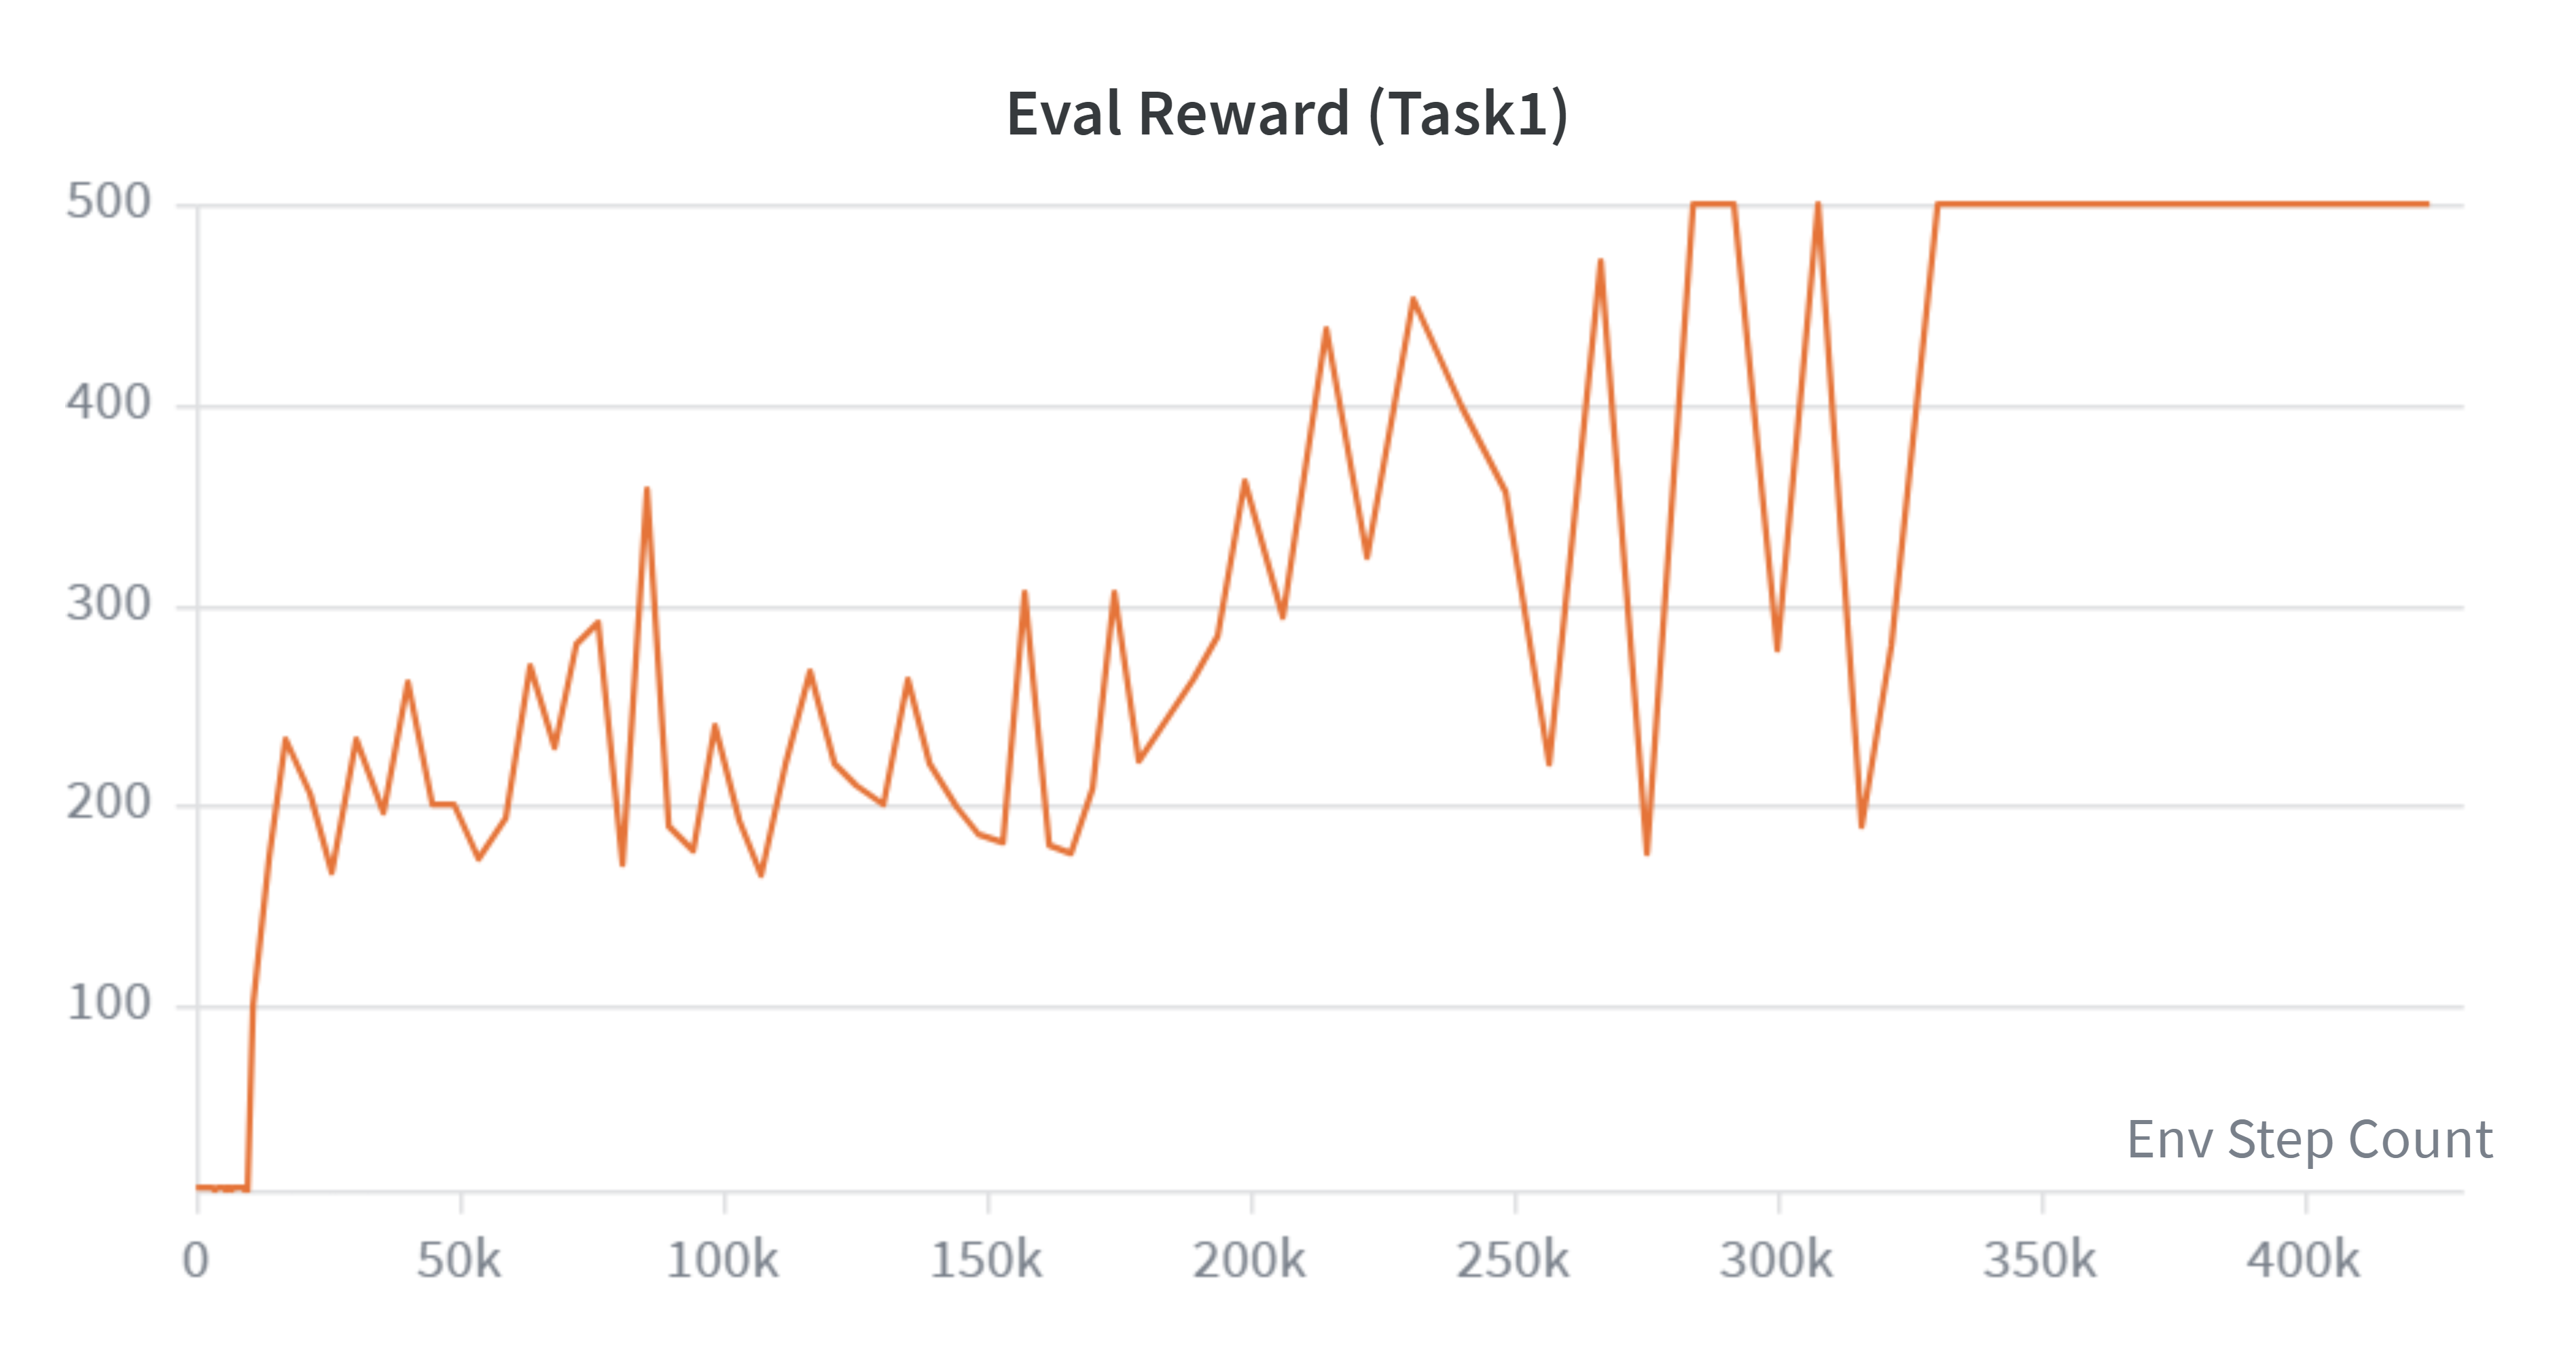
\includegraphics[width=0.65\linewidth]{W&B Chart 2026_4_28 下午12_11_37.png}
    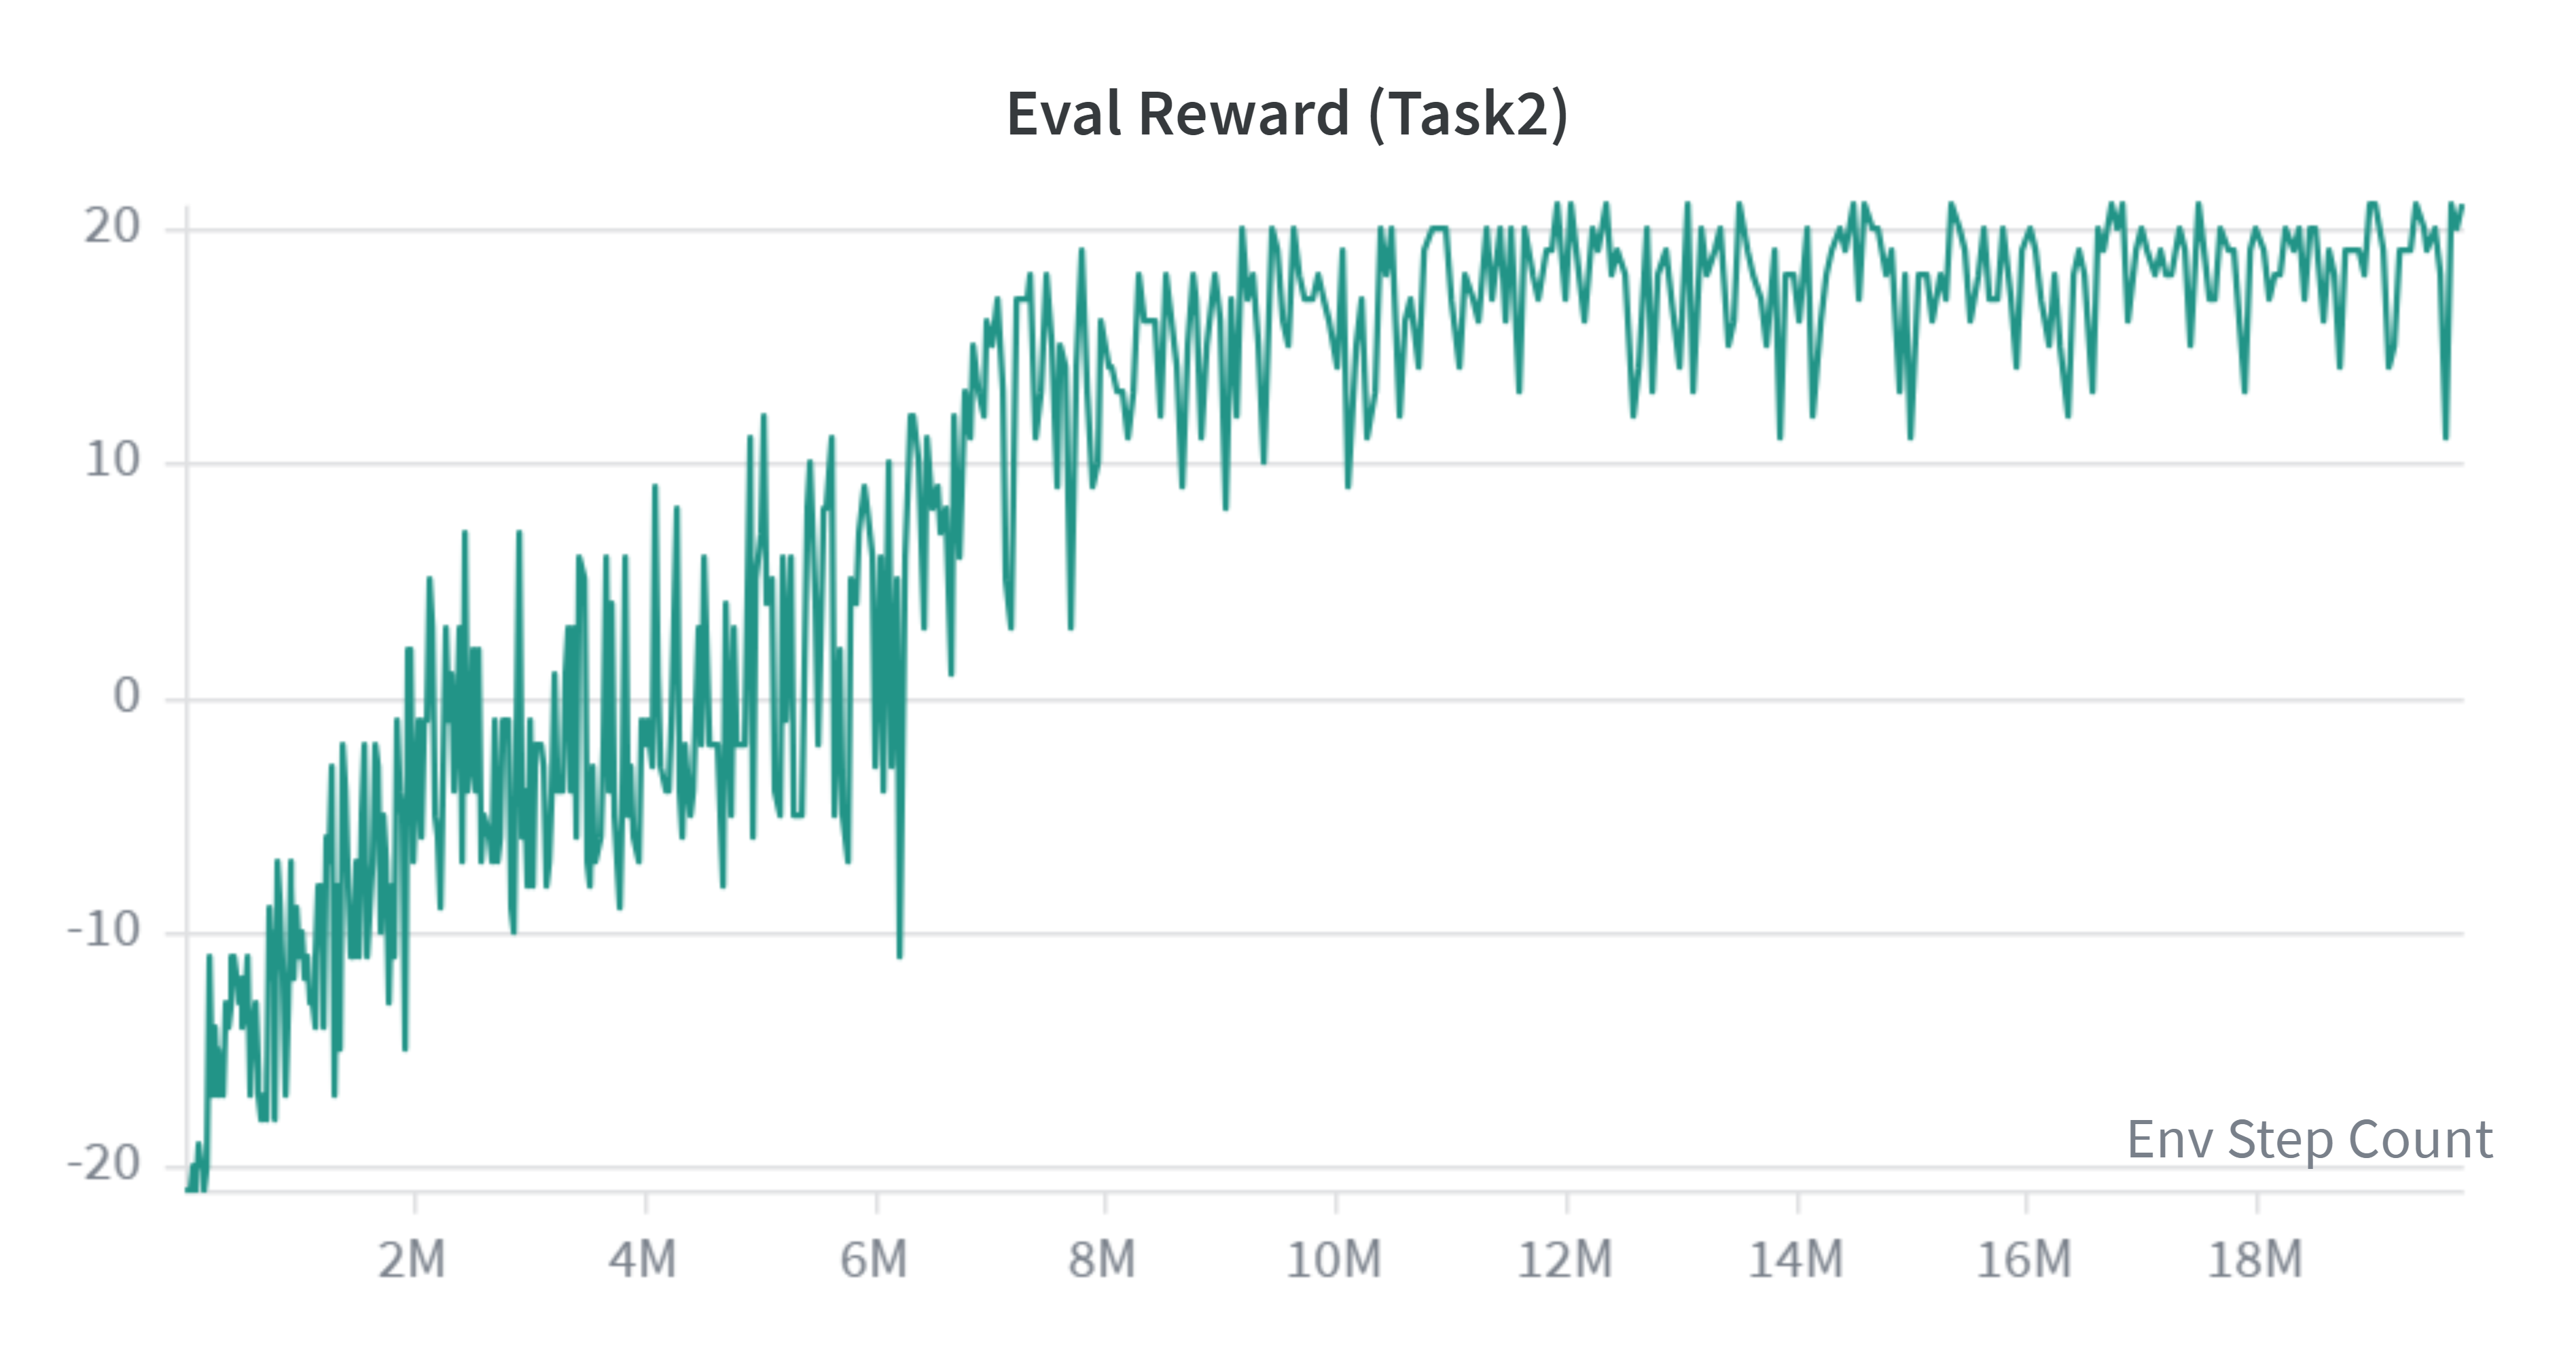
\includegraphics[width=0.65\linewidth]{W&B Chart 2026_4_29 上午11_50_41.png}
    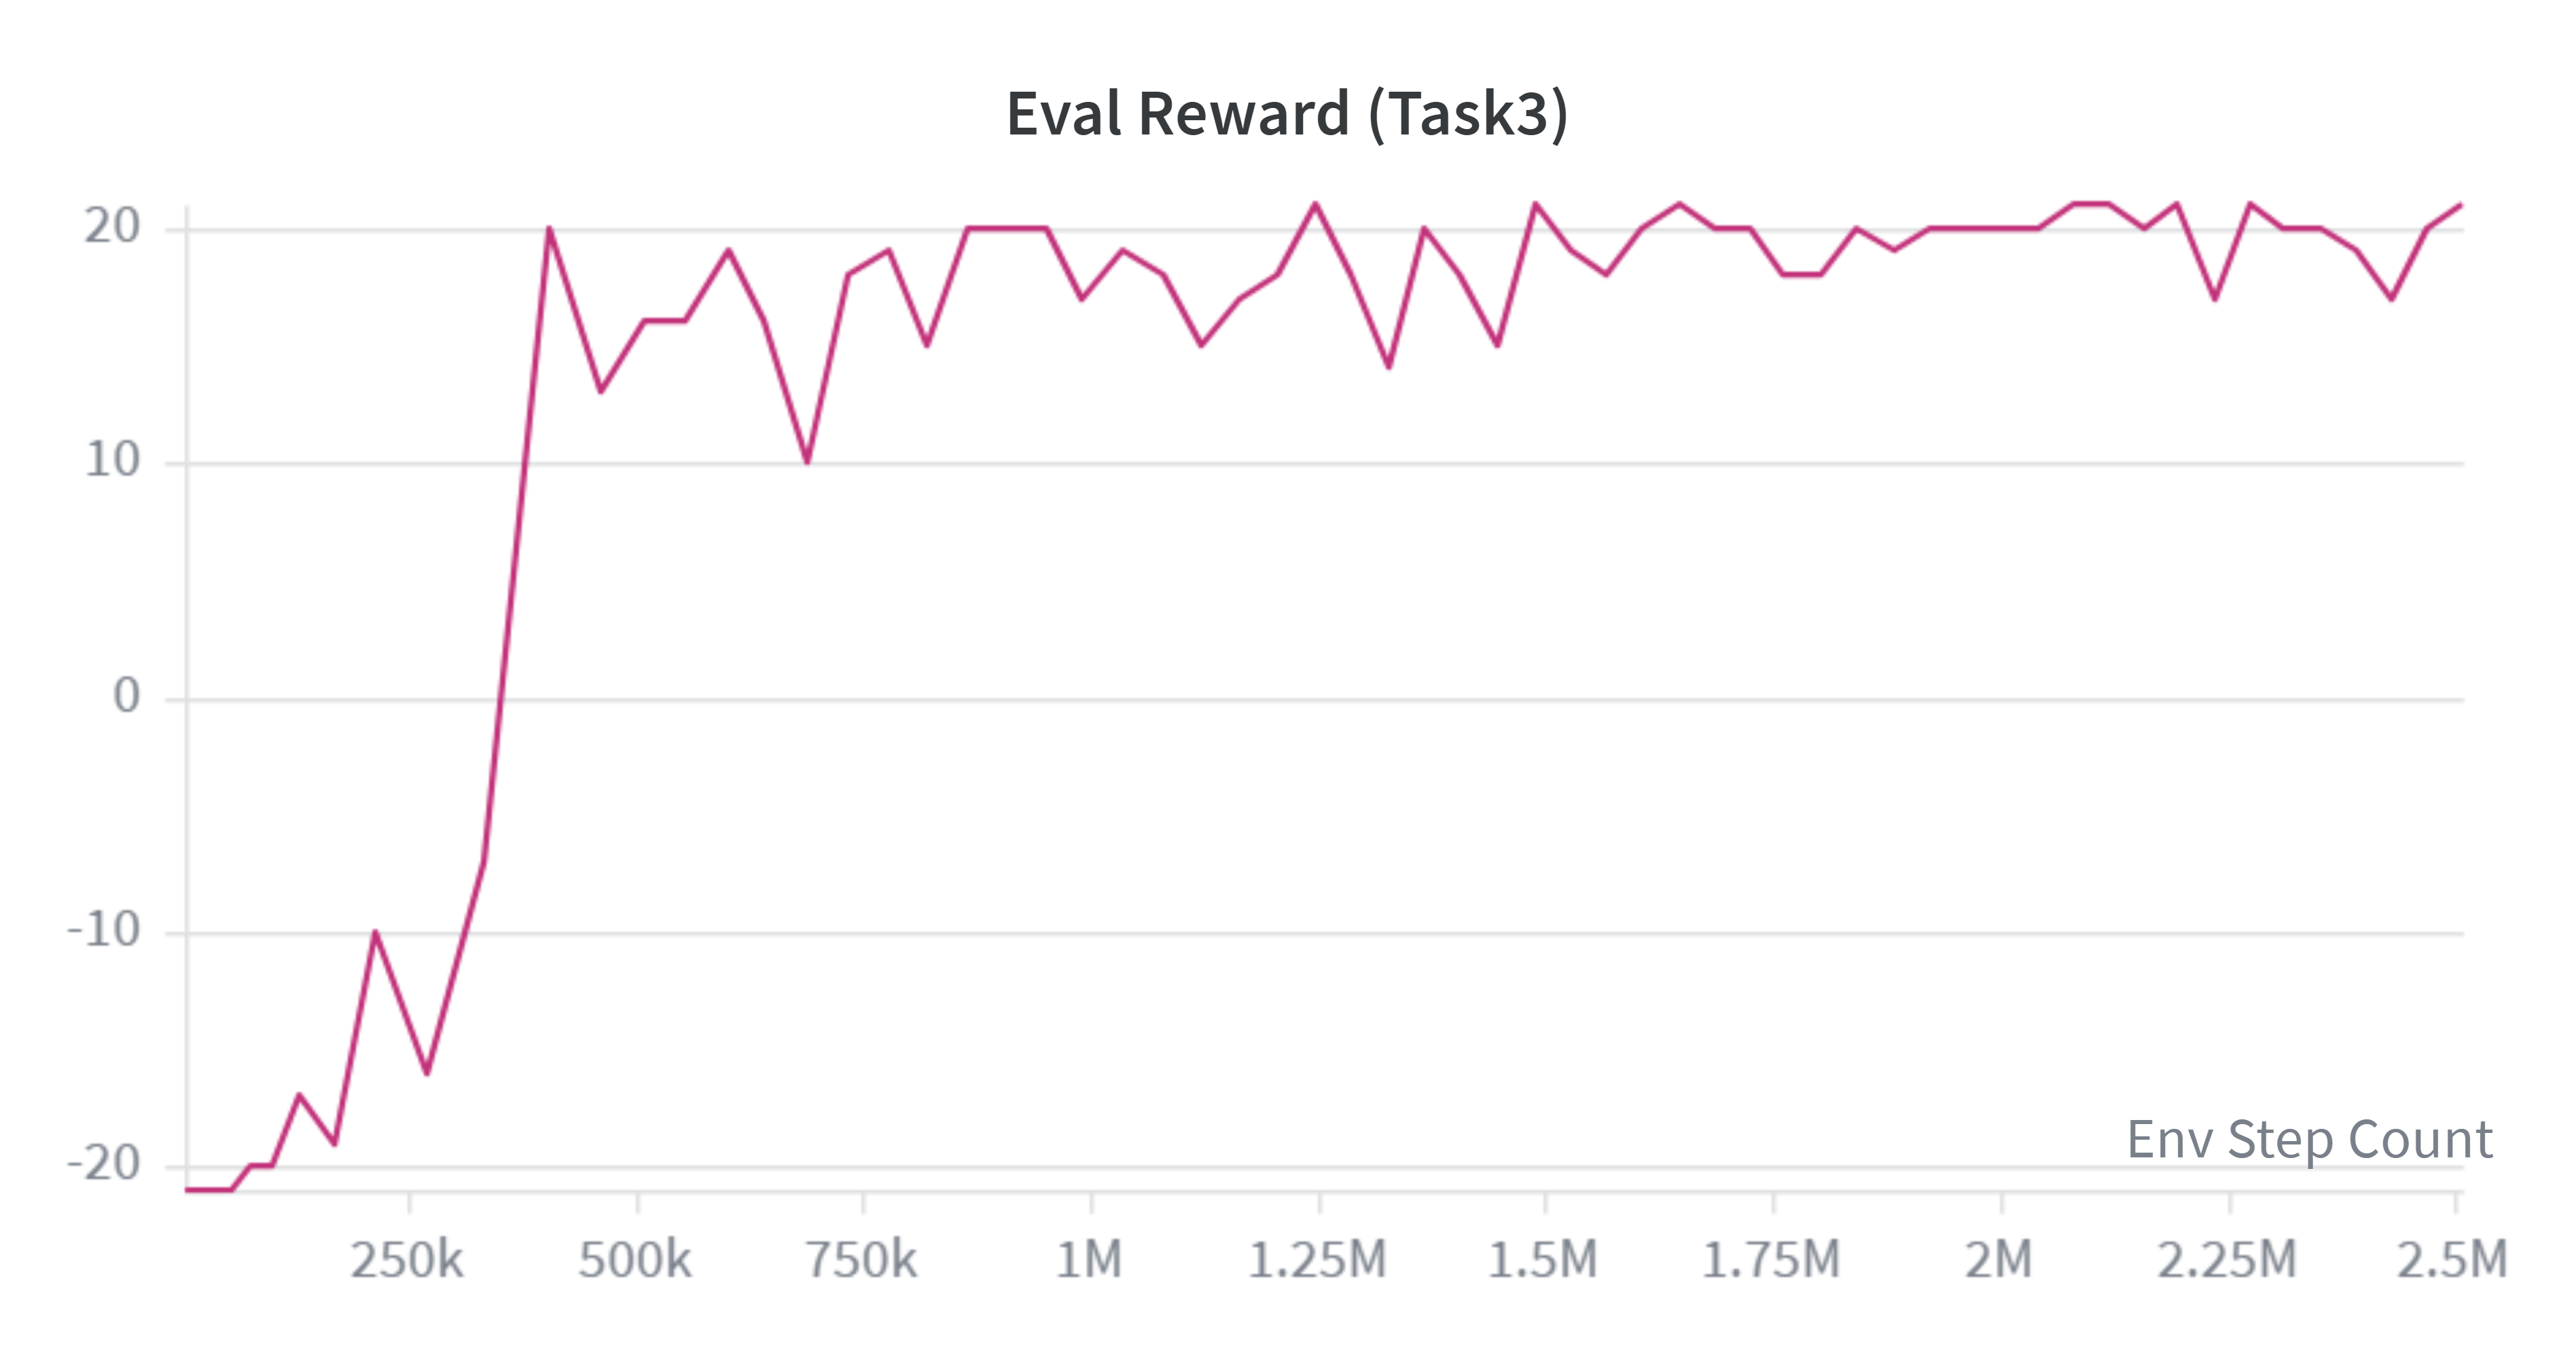
\includegraphics[width=0.65\linewidth]{W&B Chart 2026_4_29 上午11_48_20.png}
    \caption{evaluation score versus environment steps of task1, task2 and task3}
    \label{fig:placeholder}
\end{figure}

\newpage

\section{Evaluation Results}
\subsection{Task 1}

\begin{figure}[h]
    \centering
    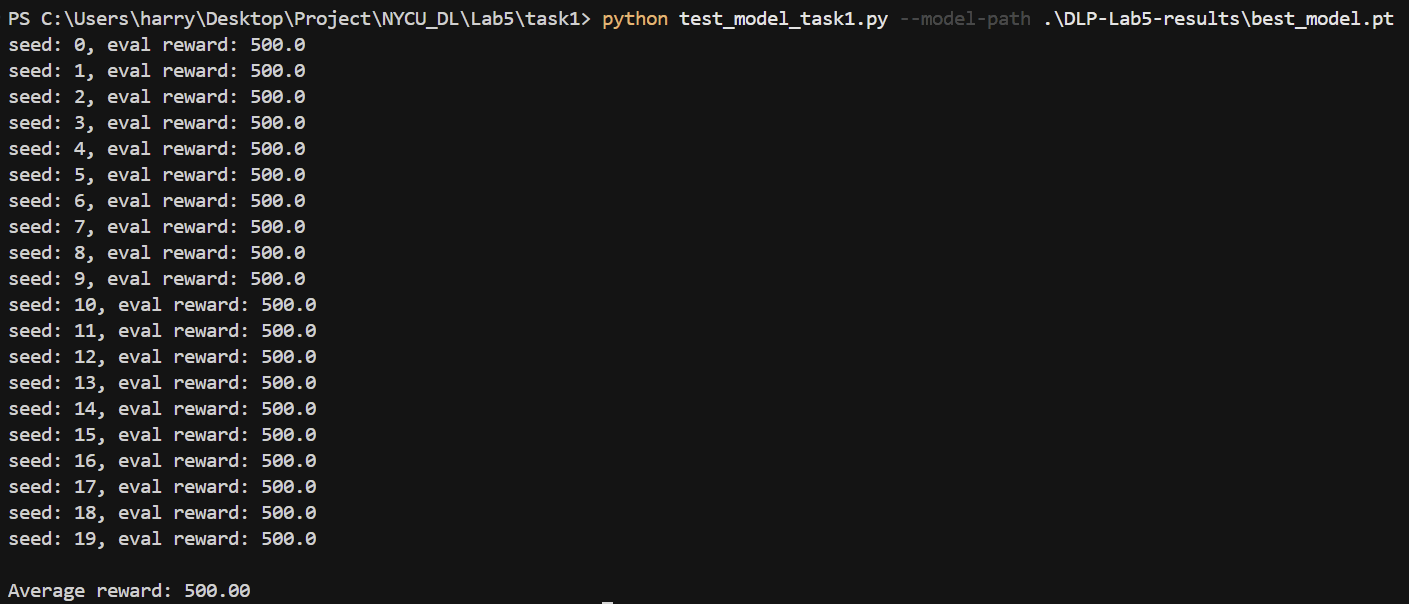
\includegraphics[width=\linewidth]{image1.png}
    \caption{Evaluation results for Task~1 (CartPole-v1): 20-episode average reward over the best submitted model snapshot.}
    \label{fig:eval-task1}
\end{figure}




The grading formula for Task~1 is (Eq.~3 in the spec):

\begin{equation}
  \text{Score percentage} \;=\;
  \frac{\min\{\text{average evaluation score},\; 480\}}{480} \times 15\%
\end{equation}

The best model achieves an average evaluation score of $\mathbf{500}$ over 20 episodes,
which exceeds the full-credit threshold of 480.
Substituting into the formula:

\[
  \text{Score percentage}
  \;=\; \frac{\min\{500,\; 480\}}{480} \times 15\%
  \;=\; \frac{480}{480} \times 15\%
  \;=\; \mathbf{15\%}
\]

\newpage

\subsection{Task 2}

\begin{figure}[h]
    \centering
    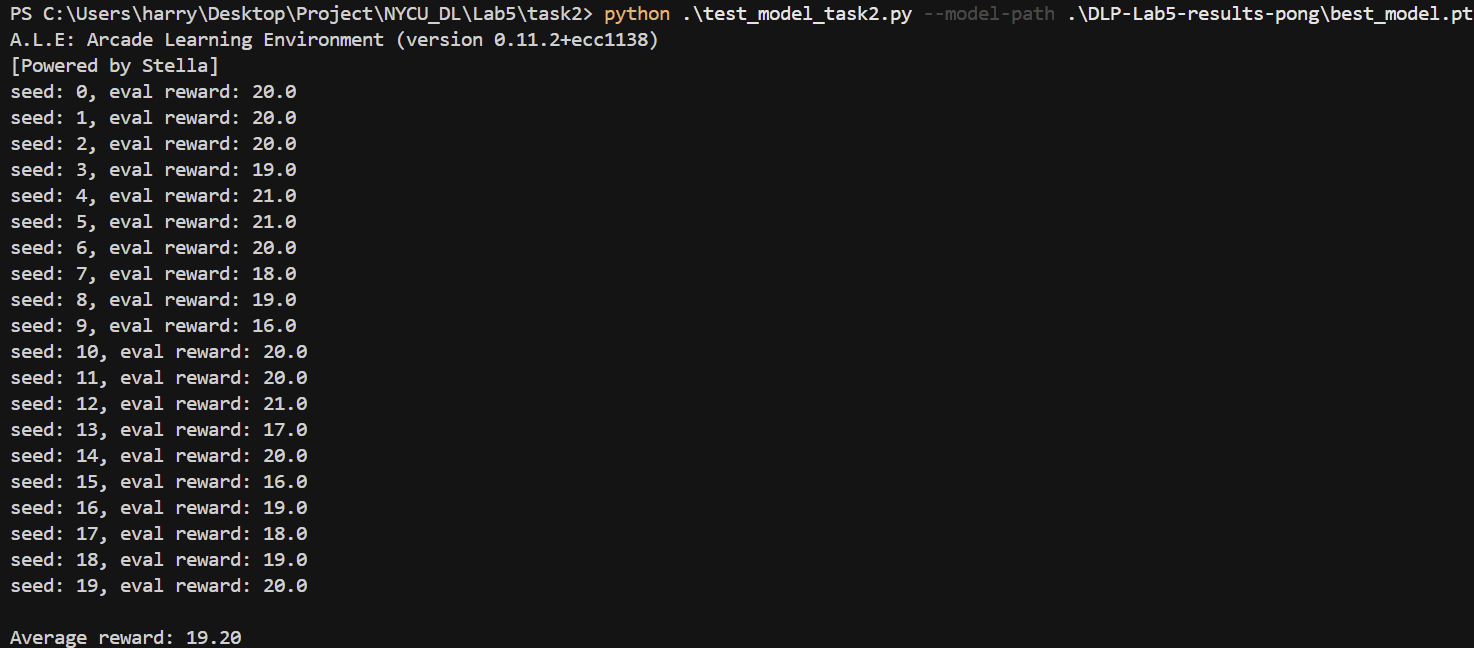
\includegraphics[width=1\linewidth]{image.png}
    \caption{Evaluation results for Task~2 (Pong-v5, vanilla DQN): 20-episode average reward over the best submitted model snapshot.}
    \label{fig:eval-task2}
\end{figure}


The grading formula for Task~2 is (Eq.~4 in the spec):

\begin{equation}
  \text{Score percentage} \;=\;
  \frac{\min\{\text{average evaluation score},\; 19\} + 21}{40} \times 20\%
\end{equation}

The best model achieves an average evaluation score of $\mathbf{19.20}$ over 20 episodes,
which exceeds the full-credit threshold of 19.
Substituting into the formula:

\[
  \text{Score percentage}
  \;=\; \frac{\min\{19.20,\; 19\} + 21}{40} \times 20\%
  \;=\; \frac{19 + 21}{40} \times 20\%
  \;=\; \frac{40}{40} \times 20\%
  \;=\; \mathbf{20\%}
\]

\newpage

\subsection{Task 3}

\begin{figure}[h]
    \centering
    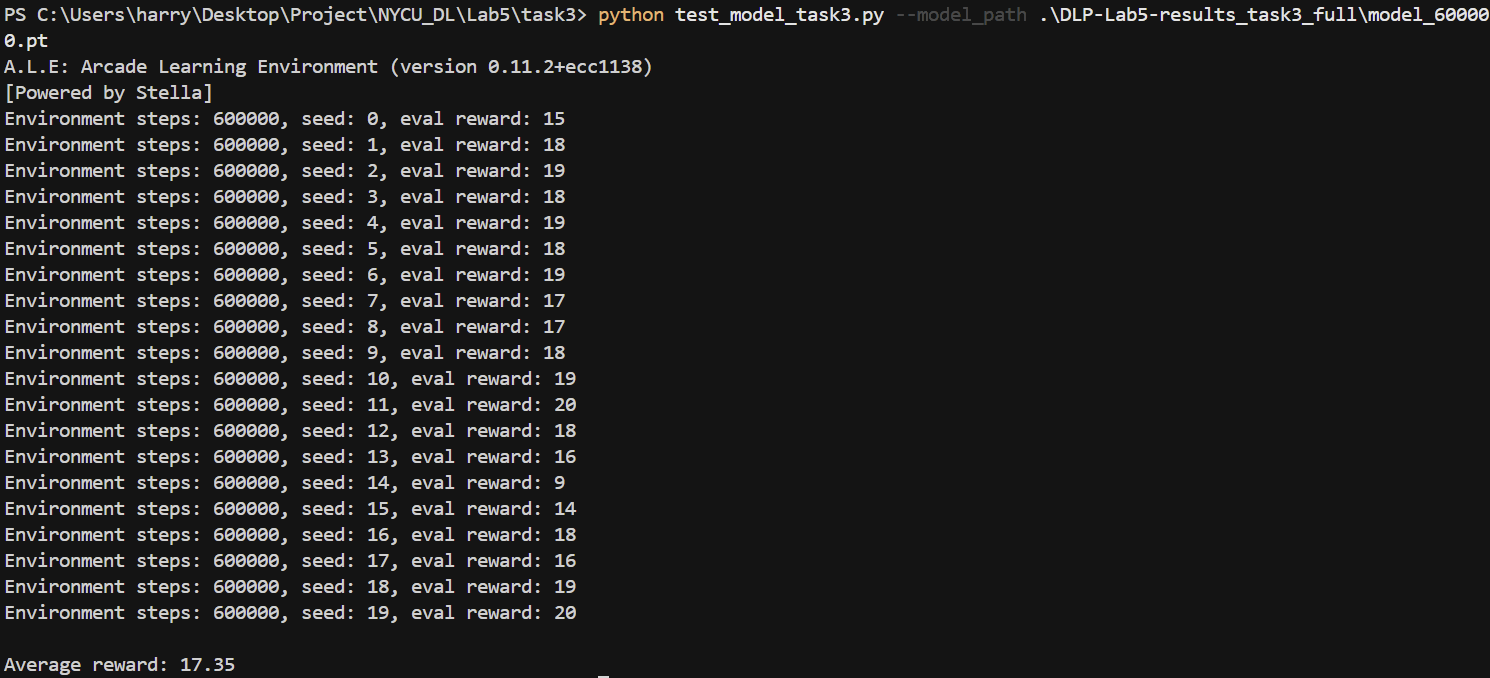
\includegraphics[width=0.75\linewidth]{image3.png}
    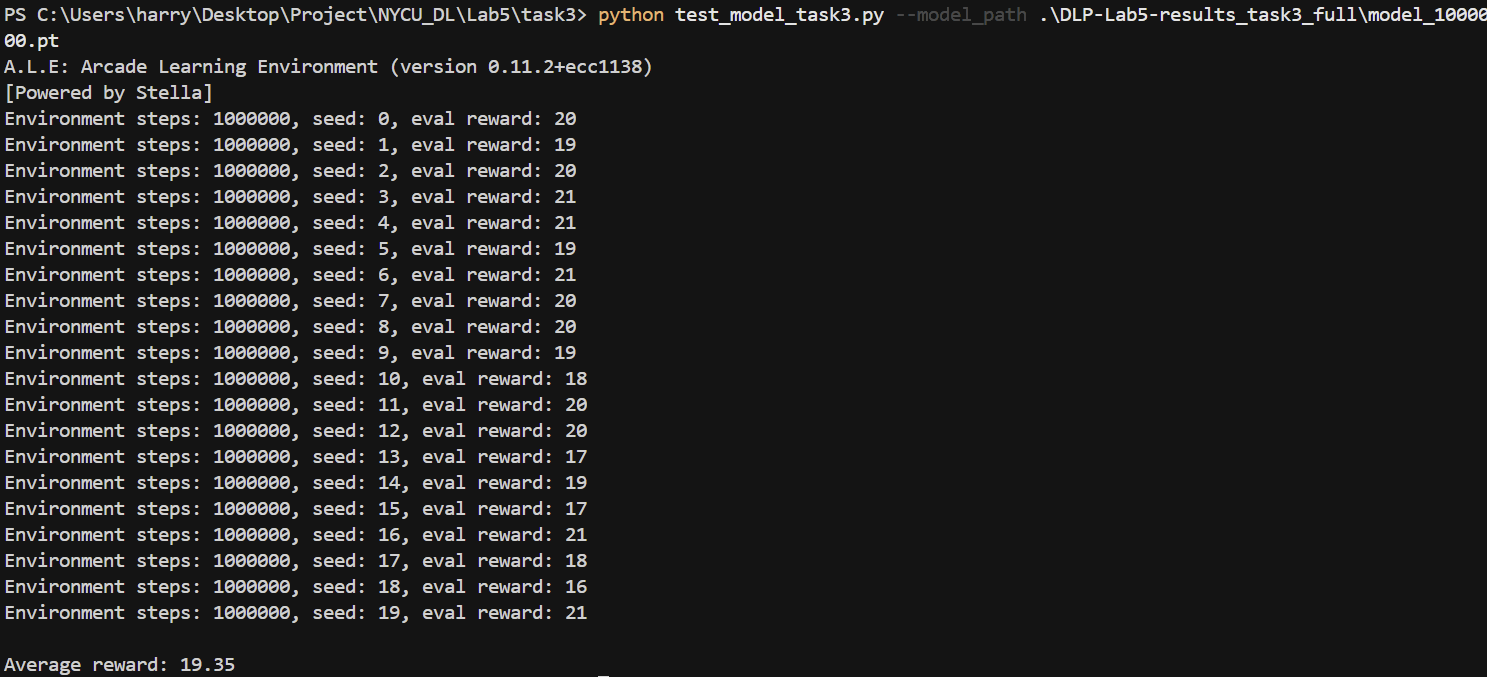
\includegraphics[width=0.75\linewidth]{image4.png}
    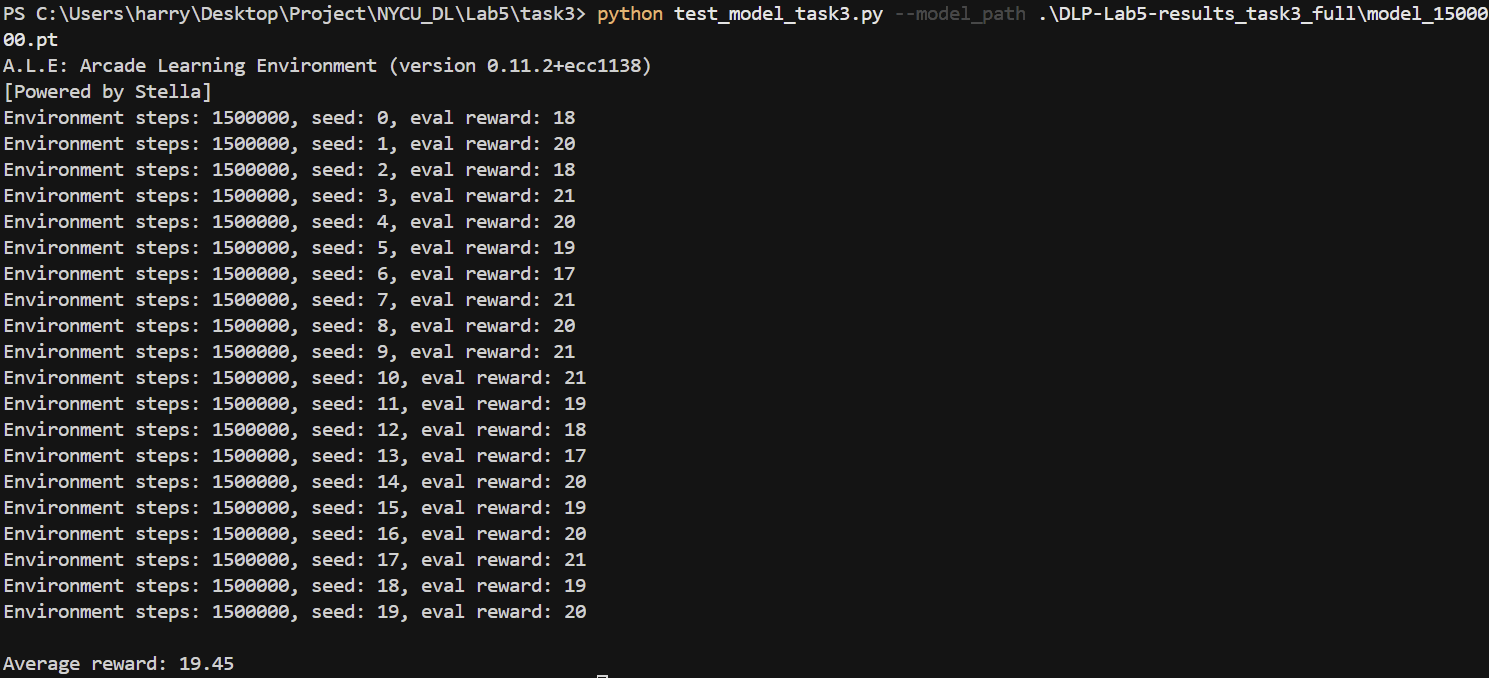
\includegraphics[width=0.75\linewidth]{image5.png}
    \caption{Evaluation results for Task~3 (Pong-v5, enhanced DQN) at 600\,k, 1\,M, and 1.5\,M environment steps}
    \label{fig:eval-task3-a}
\end{figure}

\newpage

\begin{figure}[h]
    \centering
    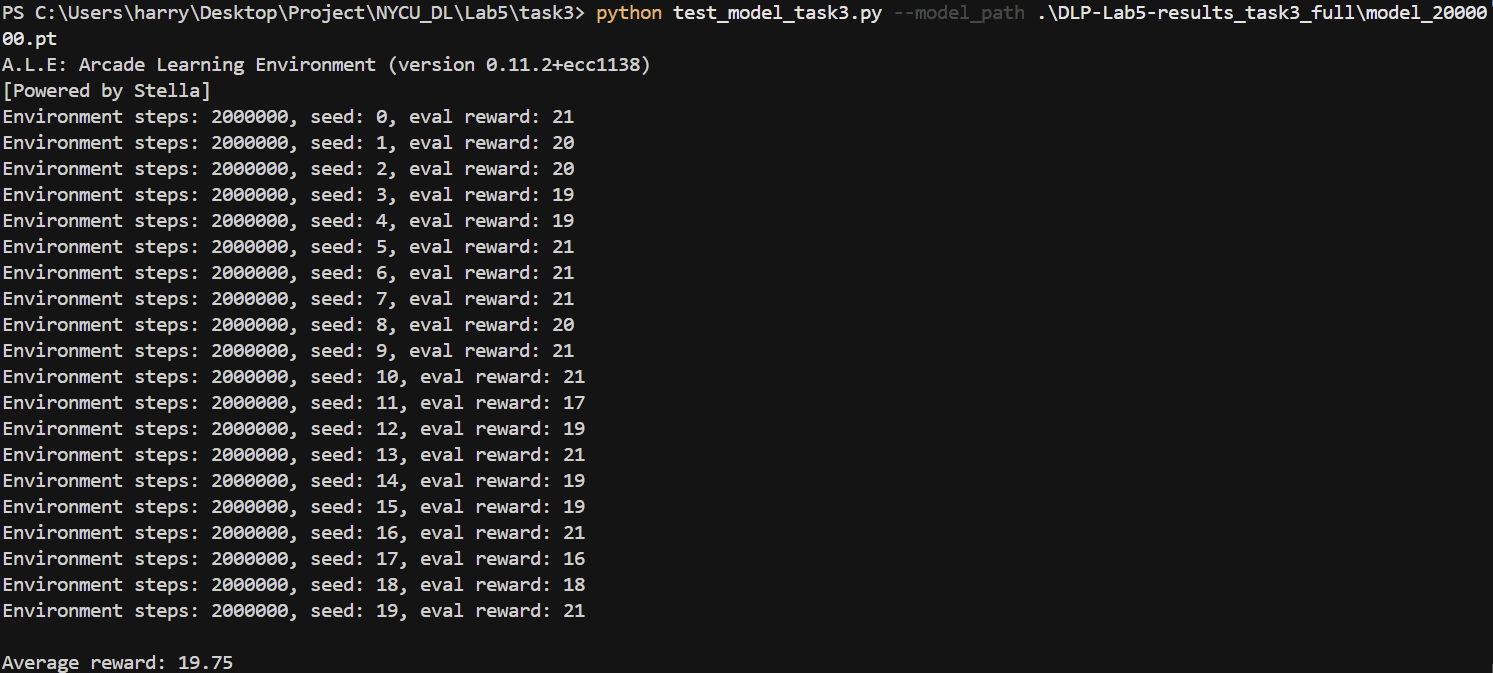
\includegraphics[width=0.75\linewidth]{image6.png}
    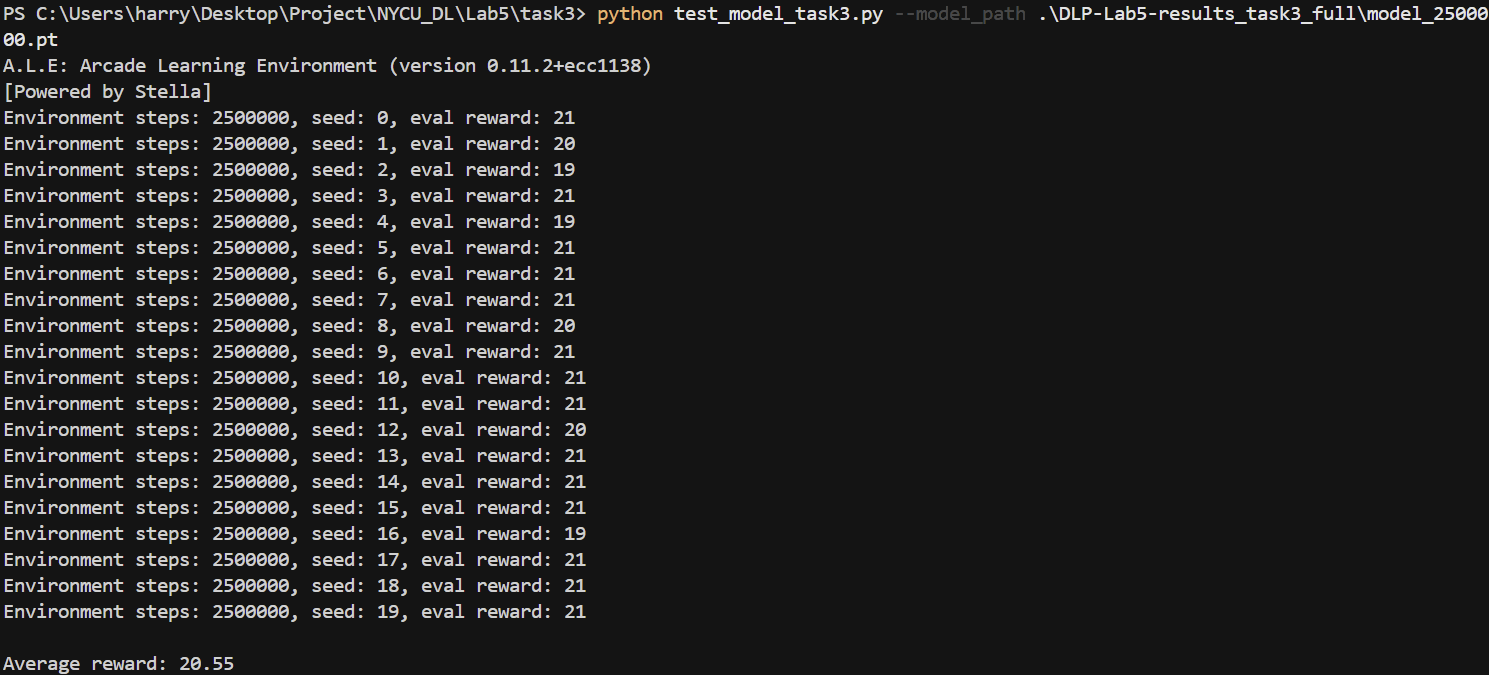
\includegraphics[width=0.75\linewidth]{image7.png}
    \caption{Evaluation results for Task~3 at 2\,M and 2.5\,M environment steps}
    \label{fig:eval-task3-b}
\end{figure}

The grading of Task~3 depends on \textbf{sample efficiency}: the fewer environment steps
required to first reach an average score of 19, the higher the score percentage.
The grading table from the spec is reproduced below:

\begin{table}[h]
\centering
\caption{Task~3 grading table (score percentage vs.\ environment steps to reach score 19).}
{\setlength{\tabcolsep}{12pt}
\begin{tabular}{lcccccc}
\toprule
\textbf{Steps to reach score 19} & 600\,k & 1\,M & 1.5\,M & 2\,M & 2.5\,M & $>$2.5\,M \\
\midrule
Score percentage & 20\% & 17\% & 15\% & 13\% & 11\% & 8\% \\
\bottomrule
\end{tabular}}
\end{table}

The 20-seed average evaluation scores at each milestone checkpoint are:

\begin{table}[h]
\centering
\caption{20-seed average evaluation reward at each Task~3 milestone checkpoint.}
{\setlength{\tabcolsep}{14pt}
\begin{tabular}{lcccccc}
\toprule
\textbf{Checkpoint} & 600\,k & 1\,M & 1.5\,M & 2\,M & 2.5\,M \\
\midrule
Average reward & 17.35 & \textbf{19.35} & 19.45 & 19.75 & 20.55 \\
\bottomrule
\end{tabular}}
\end{table}

The model \textbf{first reaches score 19 at the 1\,M-step checkpoint} (average reward 19.35).
According to the grading table, this corresponds to a score percentage of $\mathbf{17\%}$.

\newpage

\section{Analyze the sample efficiency with and without the DQN enhancements}

\begin{figure}[h]
    \centering
    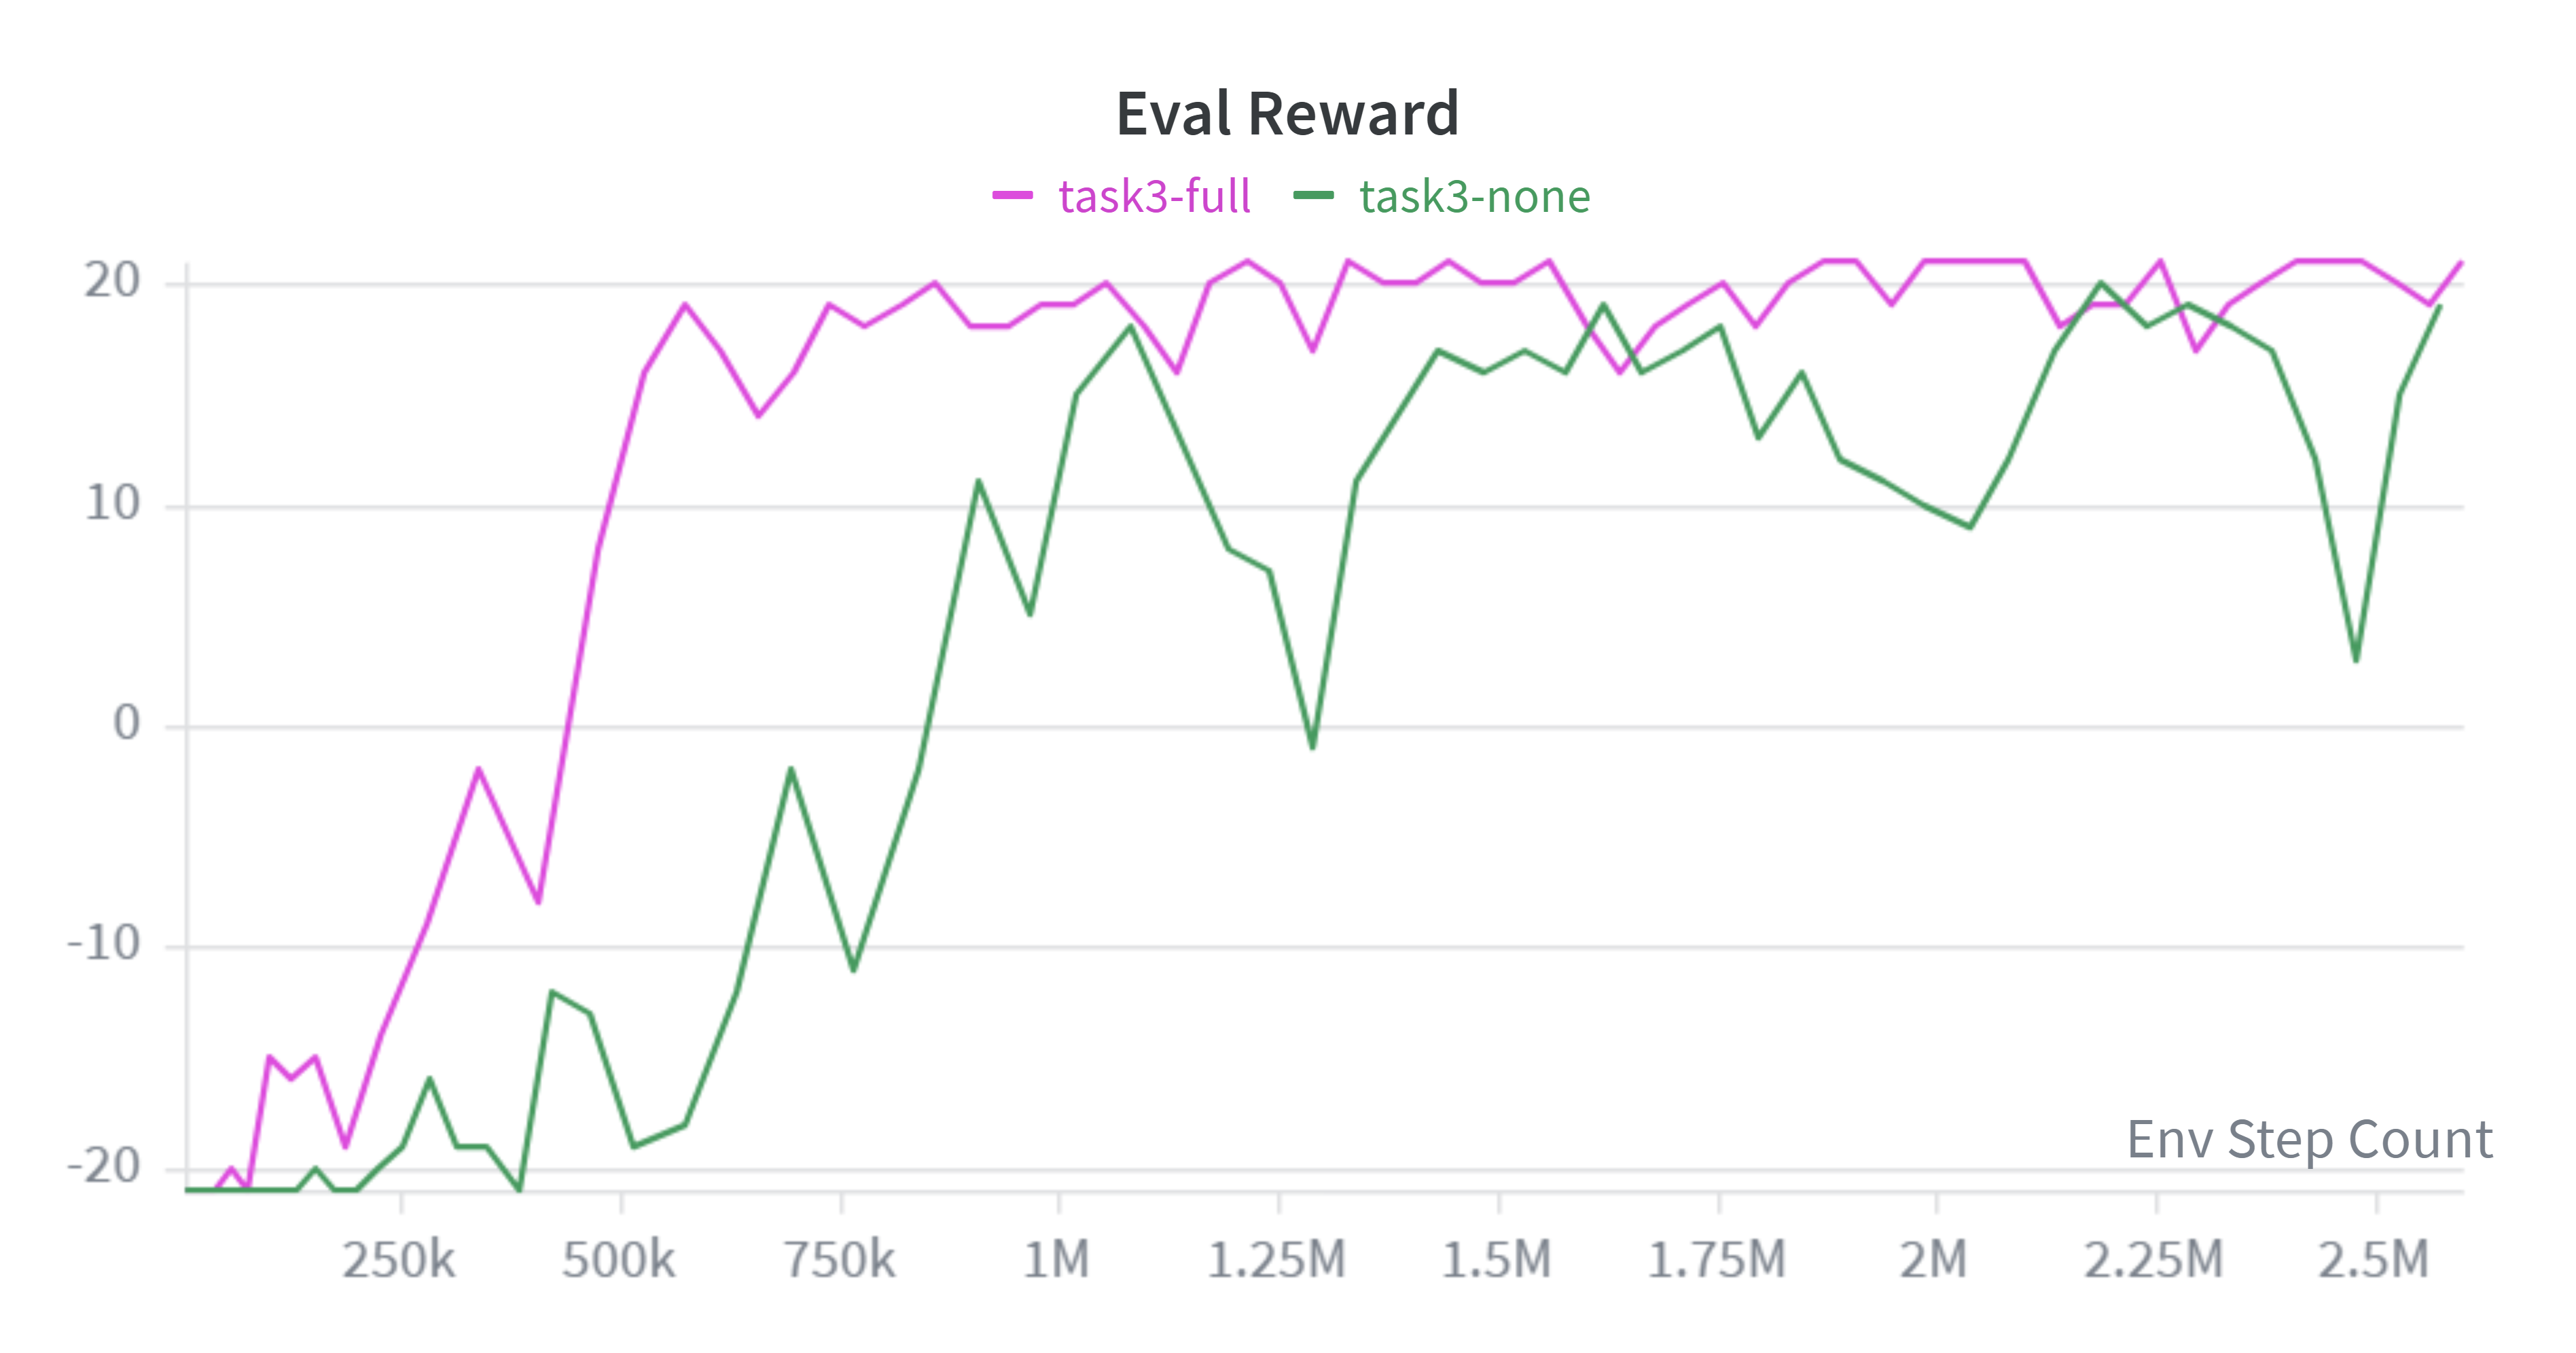
\includegraphics[width=0.75\linewidth]{W&B Chart 2026_4_29 下午5_18_44.png}
    \caption{Evaluation reward vs.\ environment steps for the enhanced agent
             (\textit{task3-full}: DDQN + PER + Multi-step $n{=}3$) and the vanilla DQN baseline
             (\textit{task3-none}) on Pong-v5.}
    \label{fig:sample-efficiency}
\end{figure}

\textit{task3-full} first crosses score 19 at around 1\,M steps and keeps climbing,
reaching 20.55 by 2.5\,M.
\textit{task3-none} needs over 2\,M steps to reach a comparable level and collapses
twice along the way due to uncorrected overestimation bias.
The gap at 600\,k is particularly stark: \textit{task3-full} already scores 17.35
while \textit{task3-none} is still near zero.
PER and multi-step return drive most of the early speed gain;
DDQN contributes mainly by keeping the converged policy stable rather than by accelerating initial learning.

\newpage

\section{Ablation study}
\begin{figure}[H]
    \centering
    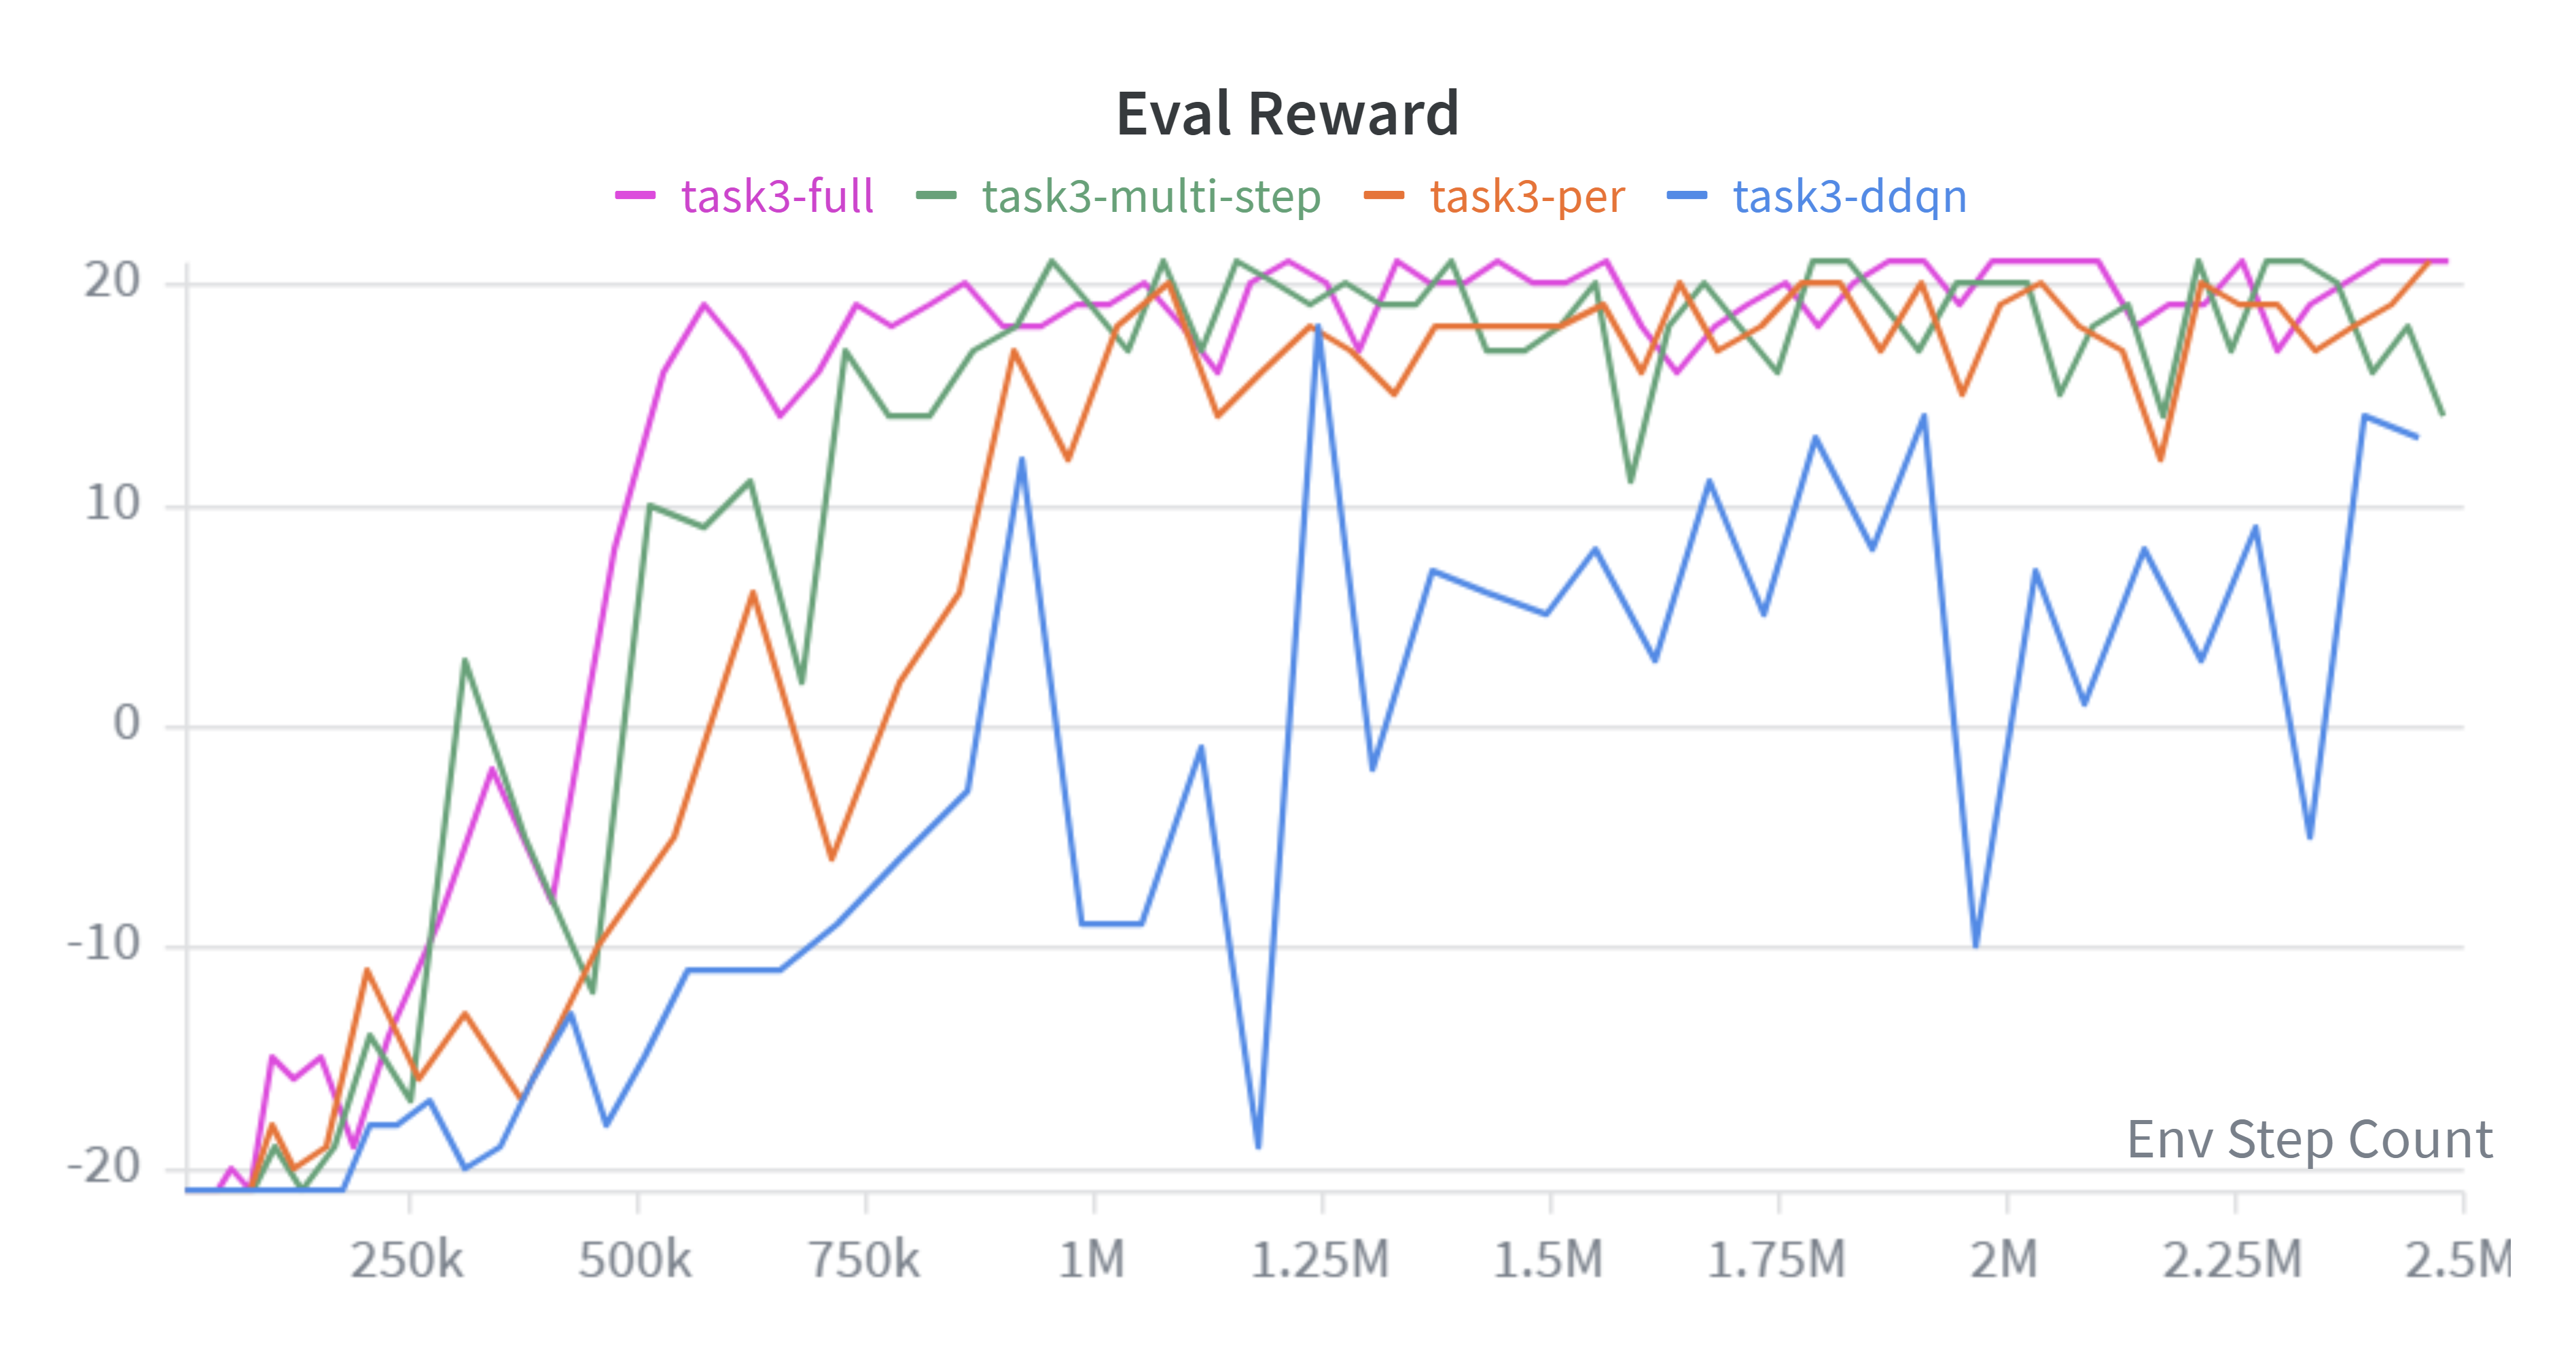
\includegraphics[width=0.75\linewidth]{W&B Chart 2026_4_29 下午10_51_33.png}
    \caption{Ablation study: evaluation reward vs.\ environment steps for each individual
             enhancement (\textit{task3-ddqn}, \textit{task3-per}, \textit{task3-multi-step})
             against the full stack (\textit{task3-full}) on Pong-v5.}
    \label{fig:ablation}
\end{figure}

Each technique is tested in isolation against the full stack (Figure~\ref{fig:ablation}).
\textit{task3-multi-step} nearly matches \textit{task3-full} on its own, reaching score 19
by $\sim$500\,k steps; multi-step return is the biggest individual driver of sample efficiency.
\textit{task3-per} converges around 1\,M steps with moderate variance, a solid but clearly
secondary contribution.
\textit{task3-ddqn} alone is the weakest: it barely climbs above 13 by 2.5\,M steps and
collapses twice, showing that DDQN does not accelerate early learning on its own;
its role is stabilising the policy once the other techniques have gotten it off the ground.
Together, the three techniques address different bottlenecks: multi-step for speed,
PER for sample coverage, DDQN for long-run stability.

Table~\ref{tab:ablation-best} summarises the best model evaluation score (average over
20 inference episodes) for each ablation configuration.

\begin{table}[H]
\centering
\caption{Best model evaluation scores (20-seed average) for each ablation configuration.}
\label{tab:ablation-best}
{\setlength{\tabcolsep}{18pt}
\begin{tabular}{llc}
\toprule
\textbf{Configuration} & \textbf{Enhancements enabled} & \textbf{Best eval score} \\
\midrule
task3-none       & None (vanilla DQN)         & 14.10   \\
task3-ddqn       & DDQN only                           & 13.50   \\
task3-per        & PER only                            & 18.95   \\
task3-multi-step & Multi-step ($n{=}3$) only           & 19.50   \\
task3-full       & DDQN + PER + Multi-step             & 20.55 \\
\bottomrule
\end{tabular}}
\end{table}

\newpage

\section{Additional analysis on other training strategies (Bonus)}

Motivated by Rainbow (Hessel et al., 2018), two additional components were evaluated on top
of the DDQN\,+\,PER\,+\,Multi-step baseline: Dueling networks and NoisyNet exploration.
Both fall short of \textit{task3-full} at every checkpoint.

\begin{figure}[h]
    \centering
    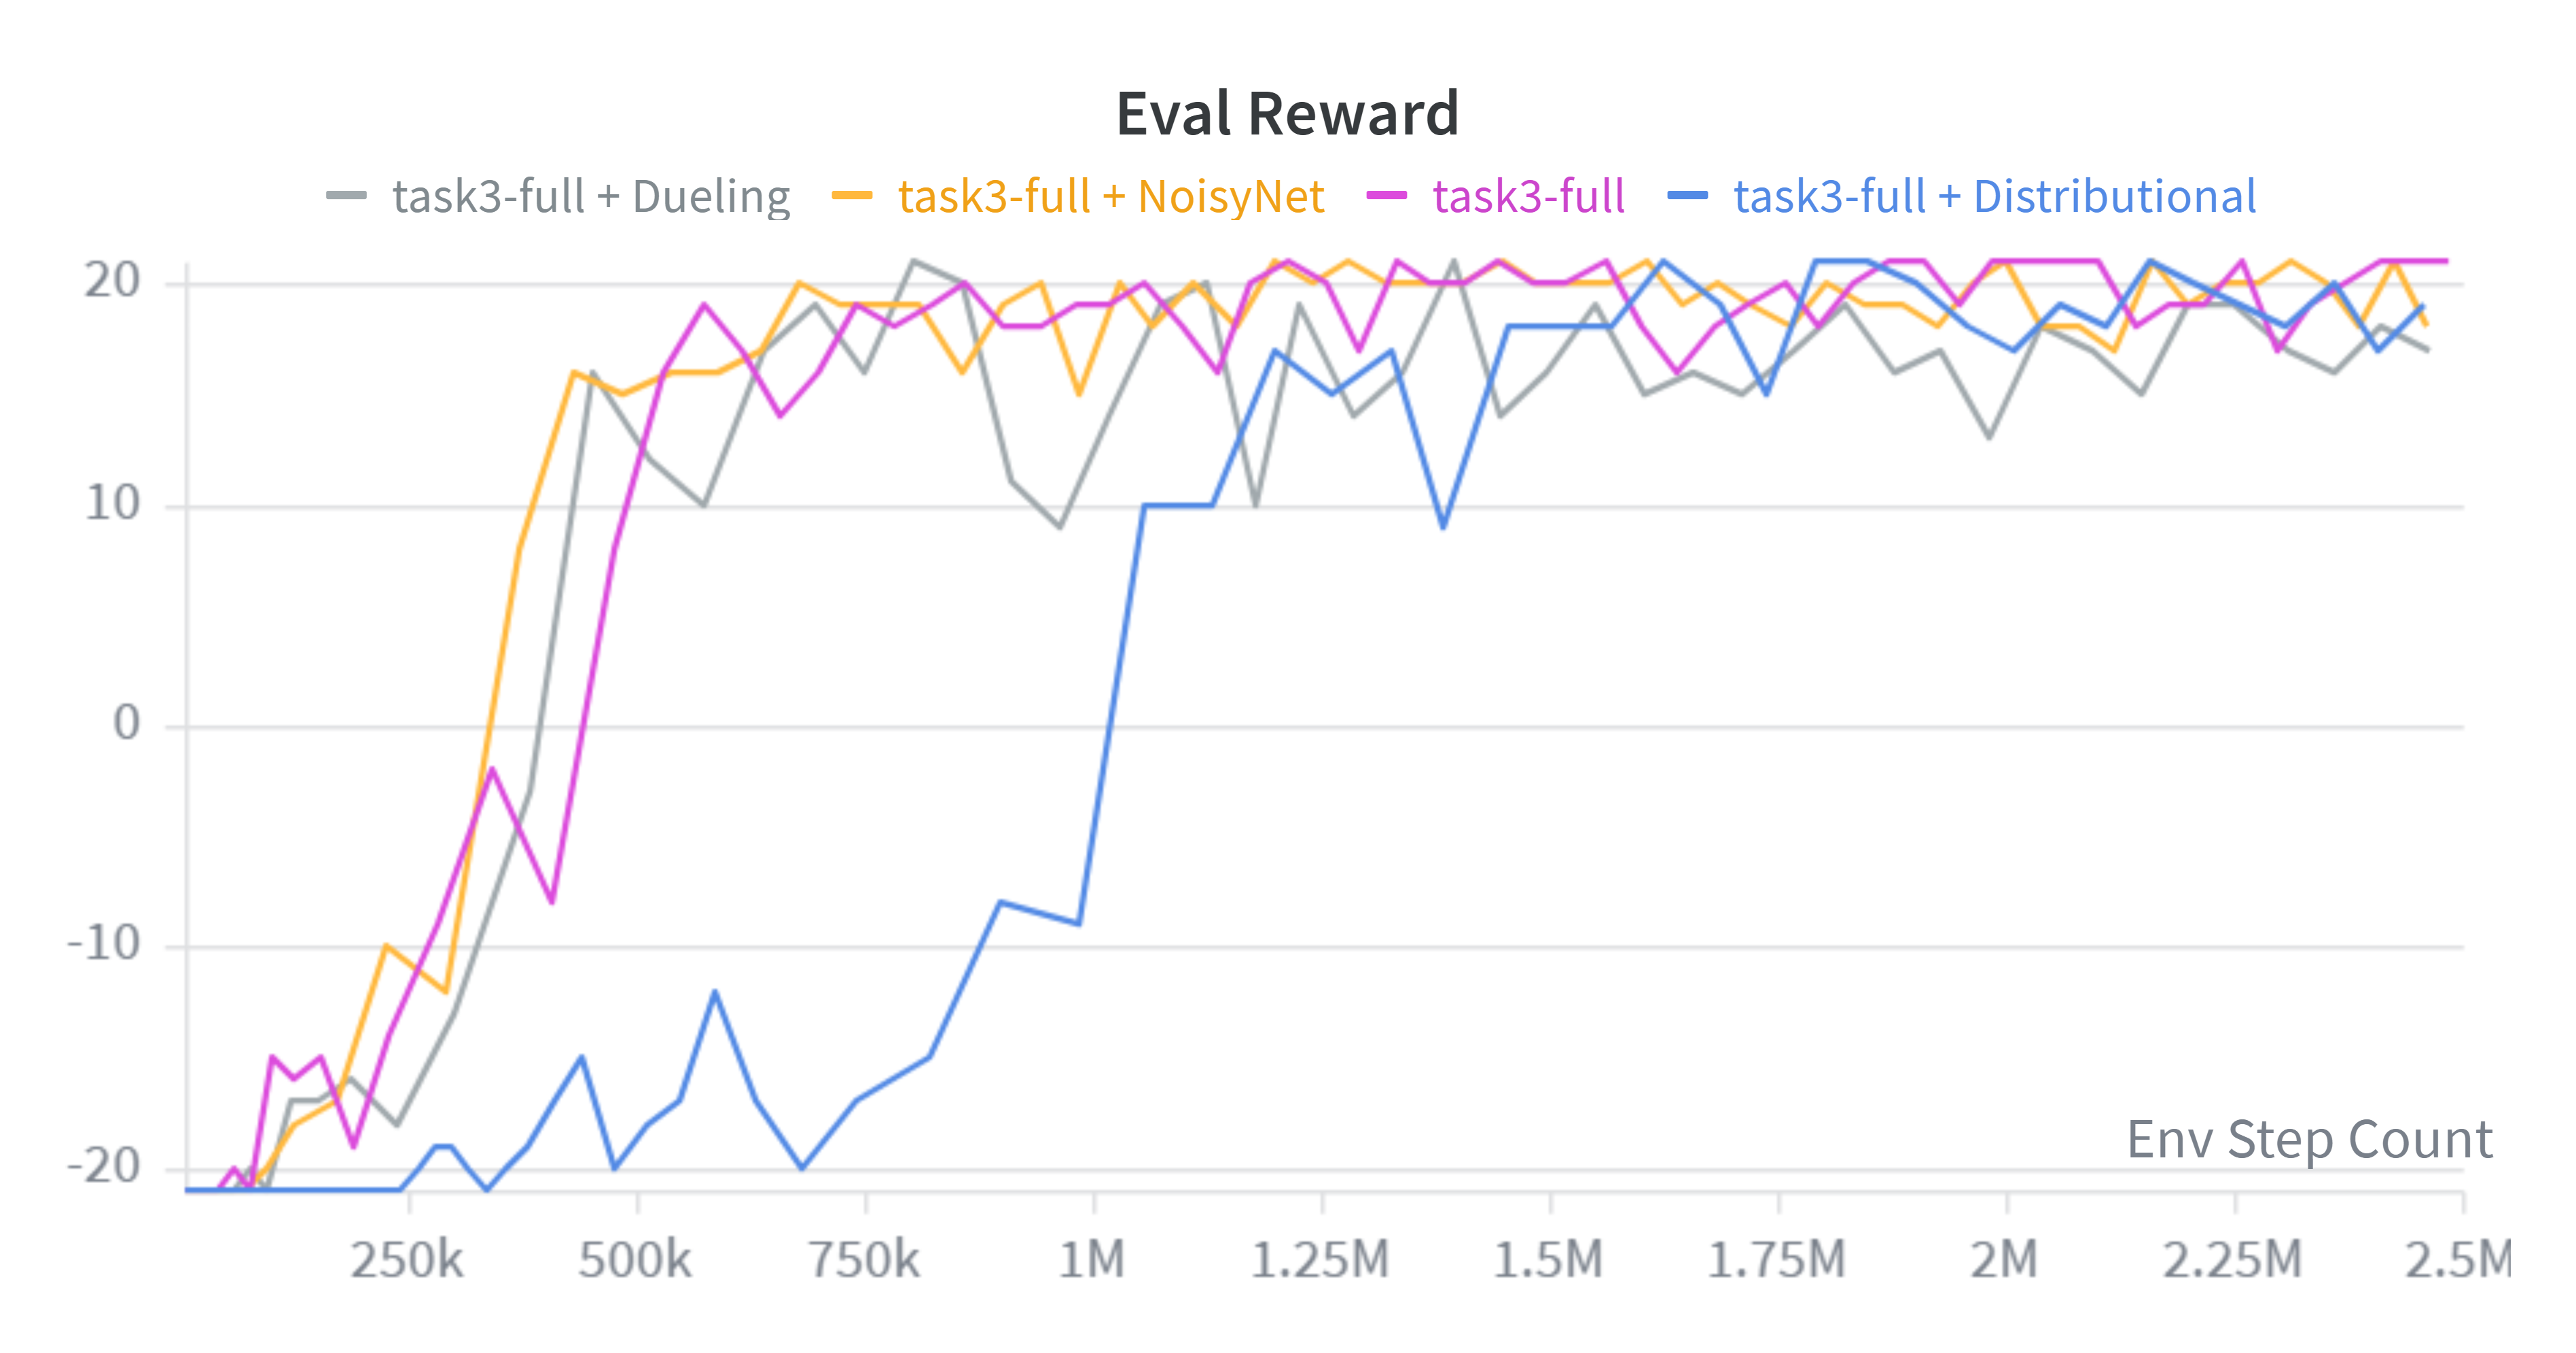
\includegraphics[width=0.75\linewidth]{W&B Chart 2026_5_1 下午6_09_04}
    \caption{Evaluation reward vs.\ environment steps for the bonus configurations
             (\textit{task3-full + Dueling} and \textit{task3-full + NoisyNet})
             against the \textit{task3-full} baseline on Pong-v5.}
    \label{fig:bonus-curves}
\end{figure}

\begin{table}[H]
\centering
\caption{20-seed average evaluation reward at each milestone checkpoint for selected configurations.}
\label{tab:ablation-milestones}
{\setlength{\tabcolsep}{10pt}
\begin{tabular}{lccccc}
\toprule
\textbf{Configuration} & \textbf{600\,k} & \textbf{1\,M} & \textbf{1.5\,M} & \textbf{2\,M} & \textbf{2.5\,M} \\
\midrule
task3-full (DDQN + PER + Multi-step) & 17.35 & 19.35 & 19.45 & 19.75 & 20.55 \\
task3-full + Dueling                 & 11.40 & 14.80 & 18.30 & 17.90 & 18.35 \\
task3-full + NoisyNet                & 16.85 & 18.65 & 19.00 & 19.20 & 18.45 \\
task3-full + Distributional          & $-17.30$ & 10.10 & 16.65 & 17.05 & 18.35 \\
\bottomrule
\end{tabular}}
\end{table}

\subsection{Dueling DQN}
Adding Dueling DQN hurts the most.
At 600\,k steps it scores only 11.40, more than 5 points below \textit{task3-full}, and
by 2.5\,M it peaks at 18.35 without ever closing the gap.
The trajectory between 1.5\,M and 2\,M (18.30 $\to$ 17.90) also suggests the policy
is not stable after converging.
The root cause is likely a conflict with PER.
Dueling splits $Q(s,a) = V(s) + A(s,a)$, so each TD error reflects a mix of inaccuracy
in the value stream and the advantage stream rather than a single clean signal.
PER was designed assuming that TD error tracks how much a transition needs to be revisited;
when that signal is noisy, priorities drift, the replay distribution skews, and early
learning slows down.
Pong compounds this: almost every state requires a decisive action, so the value stream
$V(s)$ rarely dominates and the main benefit of dueling (factoring out state value from
action advantage) barely applies.

\newpage

\begin{figure}[h]
    \centering
    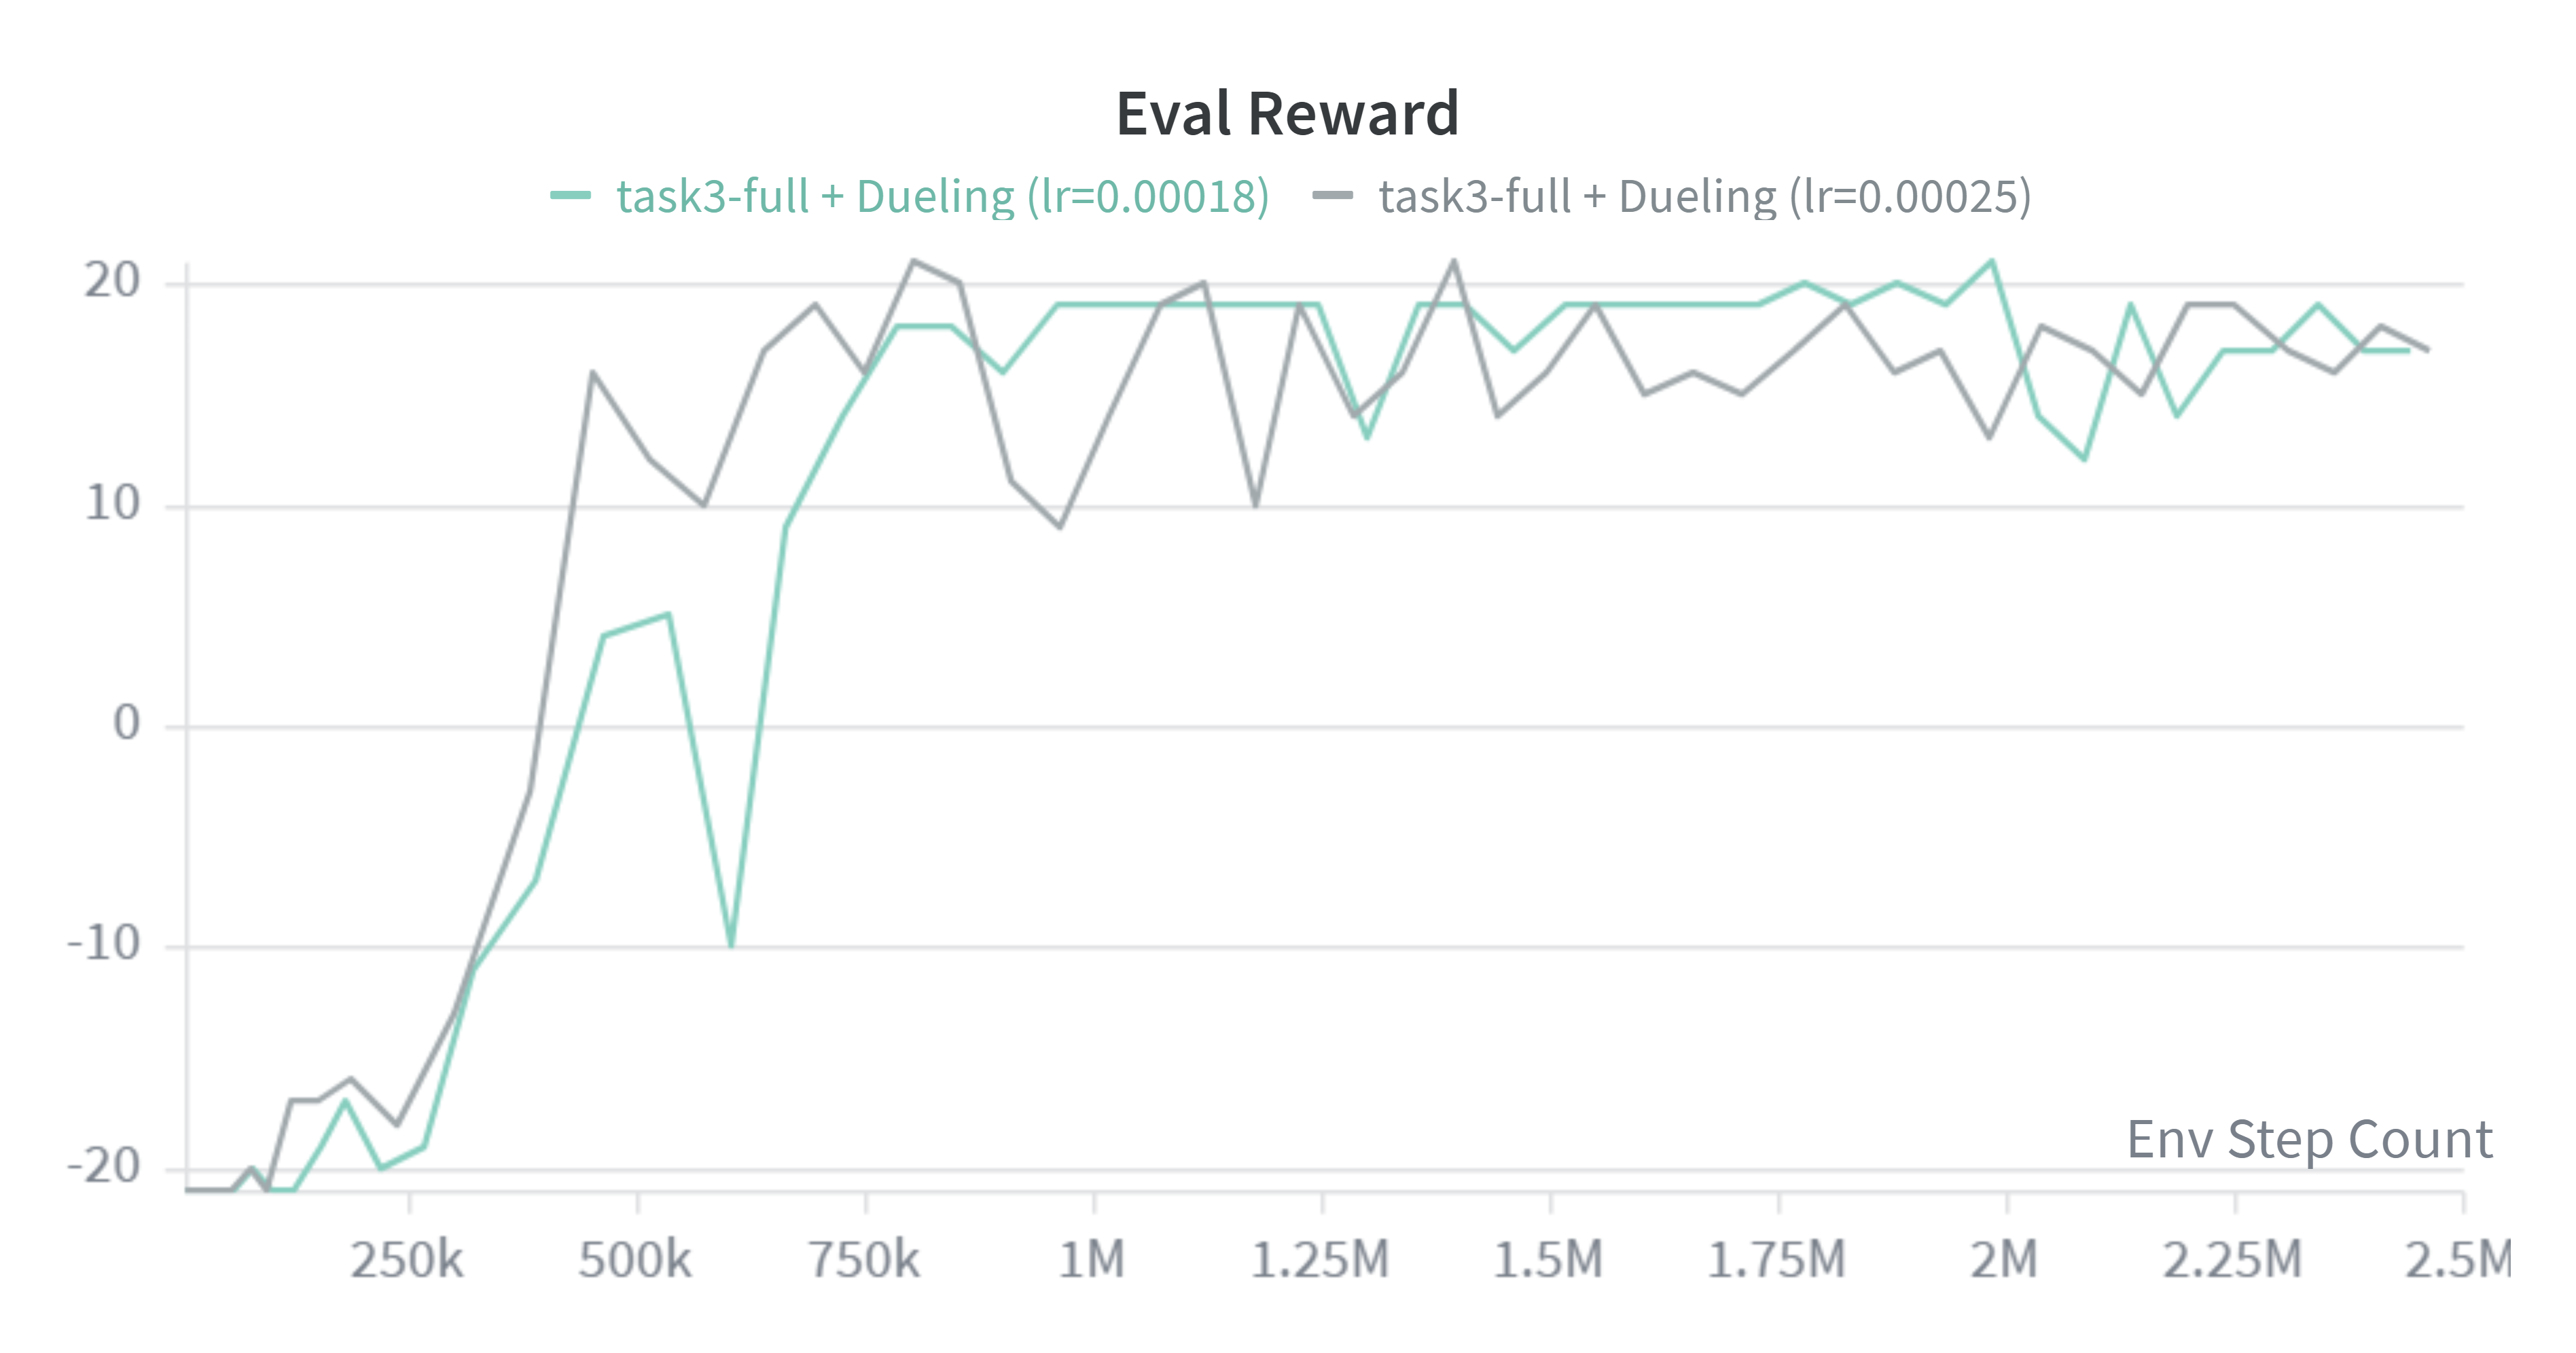
\includegraphics[width=0.75\linewidth]{W&B Chart 2026_5_1 上午11_14_09}
    \caption{Evaluation reward vs.\ environment steps for the bonus configurations
             (\textit{task3-full + Dueling(lr=0.00025)} against the \textit{task3-full + Dueling(lr=0.00018)})
             on Pong-v5.}
    \label{fig:bonus-curves-dueling}
\end{figure}

We also investigated whether an overly high learning rate was responsible for Dueling's
weaker performance.
As shown in Figure~\ref{fig:bonus-curves-dueling}, learning rate does affect both
convergence speed and training stability: the higher setting ($\text{lr} = 2.5\times10^{-4}$)
converges faster but with larger variance, while the lower setting ($\text{lr} = 1.8\times10^{-4}$)
is more stable in the later stages at the cost of slower initial learning.
Final performance is similar in both cases, suggesting that learning rate is not the
primary bottleneck for Dueling on Pong.

\subsection{NoisyNet}
NoisyNet stays much closer to the baseline but still falls short.
It reaches 19.00 at 1.5\,M and plateaus near 19.20, while \textit{task3-full} keeps
climbing to 20.55.
The idea behind NoisyNet is to replace the $\varepsilon$-greedy schedule with learnable
per-weight noise, which works best when the exploration schedule itself is the bottleneck.
In this setup the $\varepsilon$ decay was already well-tuned, so replacing it buys little.
The more significant issue is that stochastic forward passes add variance to the
Q-value estimates that PER uses to rank transitions.
That variance corrupts the priority signal, and the replay distribution never gets
as well-targeted as it does under the cleaner DDQN\,+\,PER\,+\,Multi-step baseline.

\subsection{Distributional DQN (C51)}
C51 converges noticeably slower than the baseline on Pong,
needing roughly 1.2\,M steps to reach a comparable score against around 300\,k for
\textit{task3-full}, and its final average of 18.35 stays below the baseline's 20.55.
The likely cause is that Pong's reward structure is too simple for distributional
modelling to help: each rally yields only $+1$ or $-1$, so the value distribution
is close to unimodal and MSE loss already captures it well.
The cross-entropy loss used by C51 needs substantially more samples to calibrate the
probabilities across 51 atoms, which hurts sample efficiency without providing any
representational benefit.
The advantage of distributional RL is expected to show up in environments with
sparser or more stochastic rewards, such as Montezuma's Revenge, where the richer
return distribution genuinely cannot be summarised by a single scalar.

\newpage

\subsection{Summary}
The Task~3 baseline was trained under aggressive hyperparameters chosen to converge
quickly within a limited step budget: $\text{lr} = 2.5\times10^{-4}$, PER $\beta$
annealing completed at 600\,k environment steps, and a fast $\varepsilon$ decay schedule.
These settings may have affected how fairly Dueling, NoisyNet, and C51 were evaluated,
as each component might behave differently under more conservative hyperparameters.
That said, all bonus experiments used the same baseline configuration to keep the
comparison consistent.

The results also point to an important observation about environment fit.
In a relatively simple environment like Pong, Dueling Network and C51 do not improve
performance and actually slow convergence.
This aligns with the conclusion of the Rainbow paper: the benefit of each component
is highly environment-dependent.
In games with straightforward reward structure and a small action space, architectural
additions struggle to show an advantage.
NoisyNet is the partial exception here; by improving exploration efficiency it shows
the clearest positive effect among the three, even if it still falls short of the
unmodified baseline at the 2.5\,M-step mark.

\end{document}
